\chapter{HubLink: KGQA by Graph Decomposition}
\label{ch:hublink}


This chapter introduces HubLink, a novel approach for \gls{kgqa}, representing the primary Contribution \hyperref[enum:c1]{\textbf{C1}} of this thesis. HubLink is specifically designed as a schema-agnostic and training-free method. Its core principle involves subdividing the graph into distinct subgraph structures, termed \emph{Hubs}, during an indexing phase. These Hubs facilitate source-aware information retrieval at query time, enabling the identification of provenance for the retrieved information. This characteristic is particularly valuable within scholarly literature search contexts, where traceability of findings is essential.

The structure of this chapter is organized to systematically present the HubLink framework. It begins with a high-level overview of the approach in Section~\ref{sec:hublink_overview}. Following this, Section~\ref{sec:hublink_formal_definitions} establishes the necessary formal definitions and concepts.

The subsequent sections provide a detailed explanation of the HubLink algorithm. Section~\ref{sec:hublink_data_models} introduces the core data models utilized. The process of identifying the root entities of the hub within the graph is presented in Section~\ref{sec:hublink_finding_hub_root_entities}. Section~\ref{sec:hublink_indexing} then explains the comprehensive indexing procedure, which includes the construction and storage of Hubs. Operations specific to the vector store employed for indexing and retrieval are described in Section~\ref{sec:hublink_vector_store_operations}. Section~\ref{sec:hublink_retrieval_strategies} elaborates on the two distinct retrieval strategies implemented within HubLink. The algorithmic description concludes in Section~\ref{sec:hublink_answer_generation}, which details the answer generation and source-linking mechanisms.

After presenting the algorithm, the chapter discusses broader aspects of the HubLink framework. Section~\ref{sec:hublink_design_rationale} examines the key design decisions made during development and provides their rationale. Section~\ref{sec:hublink_generality_and_chances} evaluates the applicability of HubLink to domains beyond scientific literature and assesses its scalability potential for large graphs. Considerations for maintaining index updates over time are discussed in Section~\ref{sec:updating_the_index}. Finally, an analysis of the limitations of the approach is provided in Section~\ref{sec:hublink_limitations}. 





\section{Overview}
\label{sec:hublink_overview}
% Der HubLink Retriever besitzt eine Indizierungs und Retrieval Phase. In der Indizierungsphase werden die entsprechenden Datenstrukturen vorbereitet, um in der Retrieval Phase die relevanten Informationen zu finden.

% \paragraph{Hubs} Als Hubs werden spezielle Entitäten im Graph klassifiziert, die für eine bestimmte Domäne oder Fragestellung von besonderer Bedeutung sind. Sie bündeln Informationen und bilden so eine Art Dreh- und Angelpunkt für die Suche nach relevanten Informationen. 

% \paragraph{Link} Als Link wird die Verbindung zwischen den Hubs gekennzeichnet, die während dem Retrieval Prozess aufgebaut wird. Dieser Link wird genutzt um die Informationen zwischen den Hubs zu aggregieren und so eine Antwort auf die Fragestellung zu finden.

% Der HubLink Retriever besteht aus insgesamt drei Phasen: der Indexierungsphase, der Retrievalphase und der Antwortgenerierungsphase. In der \emph{Indexierungsphase} werden die Datenstrukturen vorbereitet, um in der Retrievalphase die relevanten Informationen zu finden. In der \emph{Retrievalphase} werden zu der gegebenen Frage die relevanten Hubs  mit Informationen aus dem \gls{kg} gesucht. Zusätzlich werden die Hubs mit externen Informationen verlinkt, um so mehr Kontext zu erhalten. In der \emph{Antwortgenerierungsphase} wird für jeden Hub der als Relevant betrachtet wird, eine Teilantwort generiert. Aus der Menge an Teilantworten wird dann die finale Antwort generiert.In den folgenden Abschnitten werden wir auf die Indexierungsphase genauer eingehen. Anschließend stellen wir zwei verschiedene Strategien vor mit denen der HubLink Retriever arbeiten kann. Beide Strategien beinhalten jeweils die Retrieval- und Antwortgenerierungsphase.

% \begin{figure}[t]
%     \centering
%     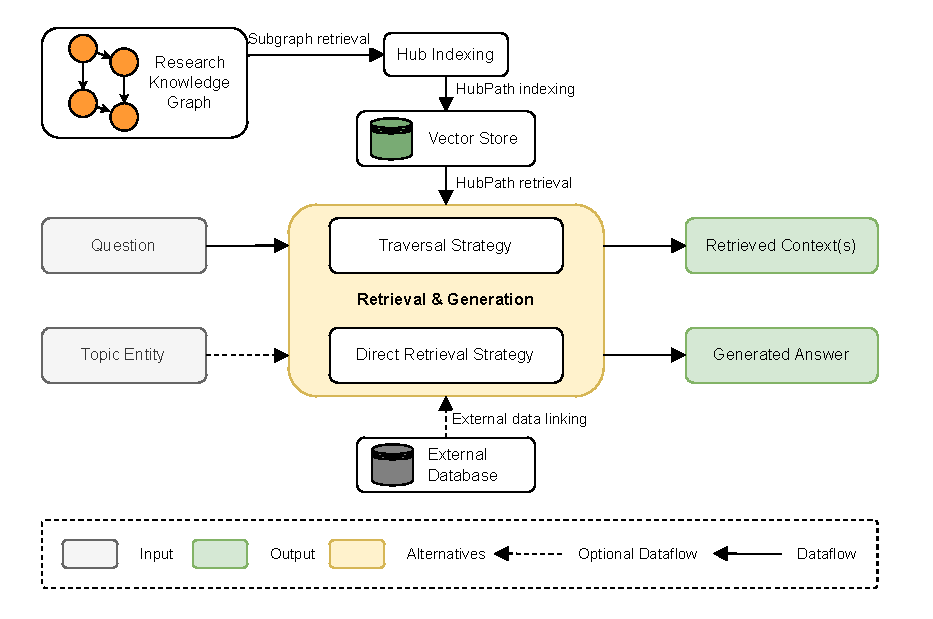
\includegraphics[width=0.95\linewidth]{figures/hublink/Hublink_figures-high_level.drawio.pdf}
%     \caption{High Level Overview of the Dataflow in HubLink}
%     \label{fig:hublink_high_level_overview}
% \end{figure}

% The dataflow of the HubLink retriever is shown in \autoref{fig:hublink_high_level_overview}. The first step of the retriever is the indexing process in which subgraphs are retrieved from an \gls{rkg}. The subgraphs consist of paths which in turn consist of triples. In the HubLink retriever, a subgraph is converted to so called \emph{HubPaths} which are stored in objects referred to as \emph{Hubs}. These are then stored in a vector store in form of low-dimensional vectors. The detailed indexing process is explained in 

This section provides an overview of our proposed HubLink approach. The purpose of this section is to illustrate the overall processes involved before diving deeper into the details in subsequent sections.

HubLink is fundamentally a \gls{grag} technique, which is characterized by its three graph-based stages: indexing, retrieval, and generation. In the following, Section~\ref{sec:hublink_indexing_process_overview} begins with the indexing process, a required preprocessing step that needs to be performed before retrieval to decompose the graph into subgraph structures referred to as \emph{hubs}. After indexing, the retrieval and generation process will be presented in Section~\ref{sec:hublink_overview_retrieval_generation}. Here, the HubLink retriever utilizes one of two different strategies to retrieve relevant data from the index. 

\subsection{Indexing}
\label{sec:hublink_indexing_process_overview}

\begin{figure}[t]
    \centering
    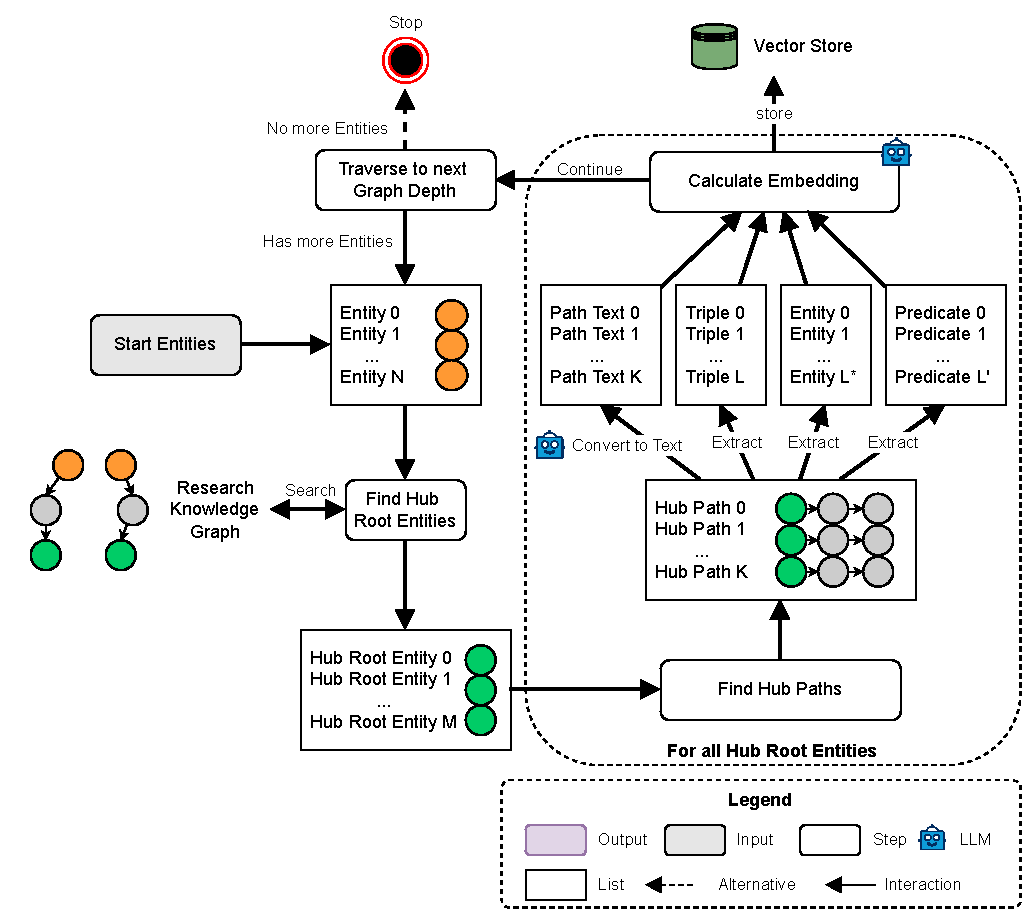
\includegraphics[width=0.93\textwidth]{figures/hublink/Hublink_figures-Overview_indexing.drawio.pdf}
    \caption[Overview of the Indexing Process]{An overview of the indexing process of HubLink showcasing how data is extracted from the \gls{kg} and stored in a vector store.}
    \label{fig:hublink_overview_indexing}
\end{figure}

The indexing process is illustrated in \autoref{fig:hublink_overview_indexing}. It begins with a set of start entities from the graph that serve as initial points for indexing. Using these entities, a search is performed with the goal of finding root entities of hubs. These are specific entities in the graph from which each hub is built. To find these roots, each possible path is traversed until either the end of the graph or until an entity in the graph is reached that is classified as the root of a hub. These identified entities are referred to as \texttt{HubRoot} objects, which are stored in a list to be processed sequentially.

For each identified \texttt{HubRoot} entity, the algorithm continues by finding and building the so-called \texttt{HubPaths}. These paths start from the \texttt{HubRoot} entity and lead to the end entities of a hub, which are either leaf nodes in the graph or other entities classified as roots of a hub. Both \texttt{HubPaths} and \texttt{HubRoot} form a \texttt{Hub} structure, which act as the central elements during retrieval.

Once the \texttt{HubPaths} of a hub are found, each path undergoes further processing before it can be indexed. First, the entire path is passed to an \gls{llm} to create a textual description of the path. In addition, an extraction of the triples, entities, and predicates from the path is performed. These pieces of information, the textual description, the triples, the entities, and the predicates, are then mapped into a low-dimensional vector space using a pre-trained embedding model. After this transformation, these vectors are stored in a vector store, which enables \gls{ann} search for fast access during the later retrieval stage. Furthermore, additional metadata are attached to each vector. This includes the root identifier of the hub for the identification of the hub to which the vector belongs and the description of the path that was generated previously by an \gls{llm}. This metadata is later required for the retrieval phase of the algorithm.

Once these hubs are indexed, the procedure repeats from the nodes in the graph that form the endpoints of each \texttt{HubPath}, provided they have not yet reached a leaf node. The indexing process stops until either the maximum number of traversal levels is reached or no new hubs are found. When the graph is updated, this update needs to be reflected in the index, which we discuss in Section~\ref{sec:updating_the_index}.

\subsection{Retrieval and Generation}
\label{sec:hublink_overview_retrieval_generation}

\begin{figure}
    \centering
    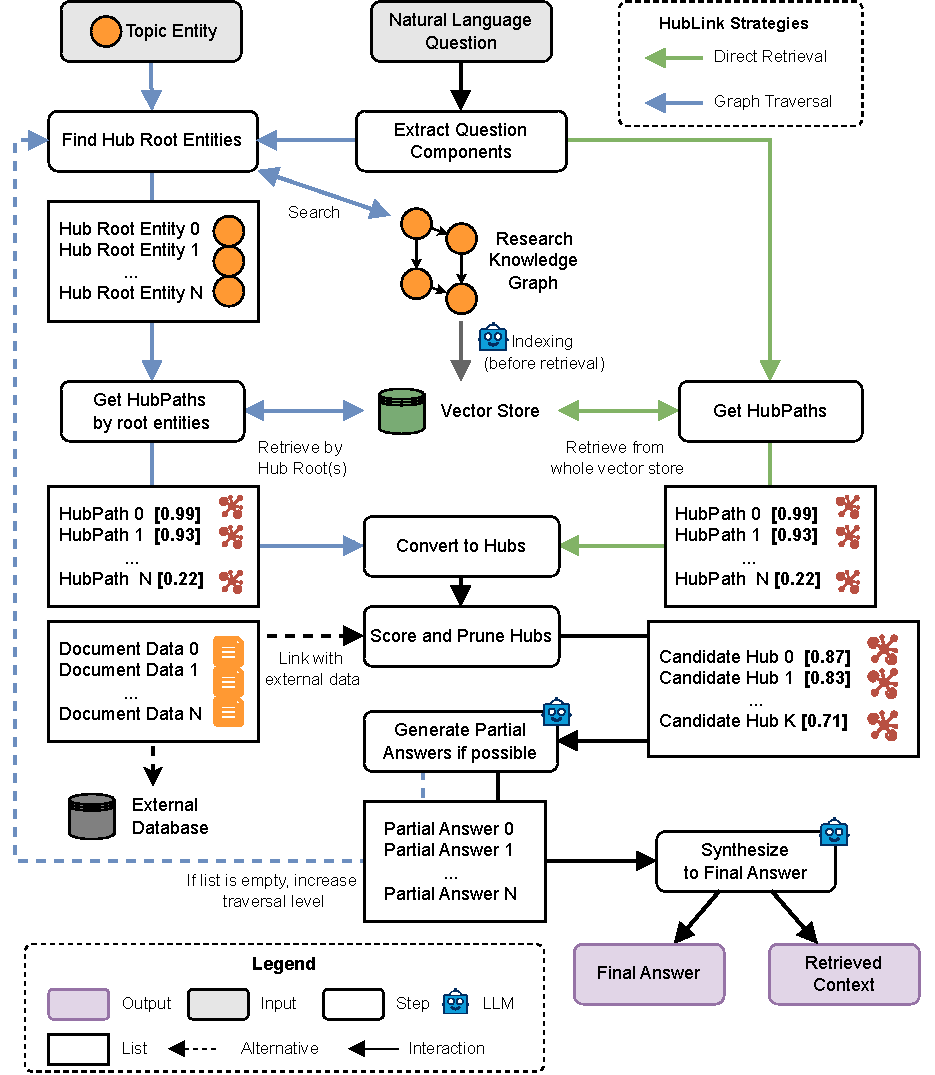
\includegraphics[width=0.98\textwidth]{figures/hublink/Hublink_figures-Overview_topic_strat.drawio.pdf}
    \caption[Overview of the Retrieval and Generation Process]{Overview of the retrieval and generation process: Two alternative strategies are depicted. The process of the direct retrieval strategy is shown with green arrows, while the graph traversal retrieval strategy is highlighted in blue.}
    \label{fig:hublink_retrieval_overview}
\end{figure}

The HubLink retrieval and generation process is illustrated in \autoref{fig:hublink_retrieval_overview}. The retriever offers two strategies for extracting relevant contexts from the \gls{kg}. The first strategy, \emph{Direct Retrieval}, performs a global search on the whole index without requiring access to the graph during retrieval. The second strategy, named \emph{Graph Traversal Retrieval}, performs a subgraph search that begins at a chosen entry point to explore the graph for the identification of relevant hubs to generate answers. The selection of the strategy involves balancing runtime and accuracy, a topic discussed later in this chapter. Both strategies differ only in certain parts of the retrieval algorithm, which we highlight in \autoref{fig:hublink_retrieval_overview} by distinguishing the paths with different colors.

The retrieval begins with an extraction of components from the question. Here, an \gls{llm} is queried to extract the most relevant parts of the question as a list. This list of components and the question itself are then transformed into vectors using the same pre-trained embedding model used in the indexing phase. Now, depending on the strategy applied, the following steps differ:

\paragraph{Graph Traversal Strategy:} In addition to the question itself, this strategy requires as input a point of entry into the graph that is referred to as \emph{Topic Entity}. The algorithm explores all paths starting at the topic entity to find \texttt{HubRoot} entities. After collecting these entities, an \gls{ann} search is performed on the vector store for each collected root entity to find \texttt{HubPaths} that are relevant to the question and contain the root entity in their metadata. This process also involves a deduplication of the paths and the application of a diversity ranker to arrive at the paths that are considered relevant to the question.

\paragraph{Direct Retrieval Strategy:} Unlike the graph traversal strategy, the direct strategy does not require a topic entity for retrieval. Furthermore, during query time, this strategy does not impose any additional queries on the graph itself. Therefore, once the components are extracted from the question, the \gls{ann} search on the vector store is directly started, which involves querying the whole store instead of querying the hubs directly, as done by the traversal strategy. Before the strategy arrives at the final \texttt{HubPaths}, it includes further techniques like clustering by hubs, deduplication of paths, and the application of a diversity ranker. 

The result of both strategies up until this point is a list of hubs with \(n\) \texttt{HubPaths} that the algorithm considers to be the most relevant to answer the question. The next step is to prune the hubs. This is done by aggregating the scores of the paths in each hub by calculating a weighted average. Only the top \(k\) hubs with the highest score are kept for the subsequent steps. 

In the next step, the \emph{Linking} process of the retriever begins. During this process, additional information is searched in an external database using the identifier of the hub, which further enriches the context of the hub beyond the knowledge collected from the graph. This could be, for example, text passages from the source publications.

By now, all necessary information about each hub has been collected. Next, for each hub, a \emph{partial answer} is generated based on the aggregated information from the hub. This is done by passing the information from the hub together with the original question in a prompt to an \gls{llm}. The \gls{llm} first checks if it is possible to provide a partial answer to the question based on this information and then provides the partial answer. If the list of partial answers is empty, no answer could be found for the question. At this step, the traversal strategy continues by traversing deeper into the graph. However, for the direct retrieval strategy, the process ends.

If partial answers have been generated, they are consolidated into a final answer. This is done by passing the partial answers to the \gls{llm} along with the original question. The \gls{llm} then generates the final answer based on this information. 


\section{Formal Definitions}
\label{sec:hublink_formal_definitions}

This section lays the formal foundation for the HubLink approach by providing definitions for the key concepts and data structures used throughout the approach. In the following, we first describe the underlying graph model to which the approach is applied. Then, we formally characterize the core elements specific to HubLink: \texttt{EntityWithDirection}, \texttt{HubRoot}, \texttt{HubPath}, \texttt{Hub}, and \texttt{HubVector}. These definitions are the prerequisites for the detailed algorithmic explanation in the following sections.

\subsection{Research Knowledge Graph (RKG)}

The underlying knowledge base is a \acrfull{rkg}, which is represented according to the \gls{rdf} standard \cite{wood_rdf_2014}. An \gls{rdf} graph provides a machine-readable semantic framework for describing ontologies, where information is expressed in the form of triples. The graph stores scholarly data where the triples capture not only bibliographic metadata (e.g., authors, dates, publishers) but also detailed relationships between scientific artifacts, for example, contributions of authors or publications. The formal definition of such an \gls{rdf} graph is provided in Section~\ref{sec:fundamentals_knowledge_graphs} and will not be repeated here.


\subsection{EntityWithDirection: Directed Graph Node}

An entity \( e \in E \) represents a node in the \gls{rdf} graph \( G \), where \( E \) is the set of all entities in the graph. Formally, the set of entities is defined as:
\[
E = \{ e \mid (s, p, o) \in G,\ e \in \{s, o\} \}.
\]

We define a path \( \mathcal{T} \) as a sequence of \( n \) triples, \( \mathcal{T} = [t_1, t_2, \ldots, t_n] \) where \( n \ge 1 \) and \( t_i = (s_i, p_i, o_i) \in G \) for all \( 1 \le i \le n \). This sequence represents a directed traversal through the graph \( G \), where adjacent triples are connected via shared entities.

When traversing such a path \( \mathcal{T} \), arriving at an entity \( e \) via the final triple \( t_n = (s_n, p_n, o_n) \) requires understanding the context: specifically, the path taken and whether \( e \) served as the subject or object. To capture this context, we introduce the \texttt{EntityWithDirection} structure. This structure associates an entity \( e \) with the specific path \( \mathcal{T} \) that ends at the entity, along with a direction indicator specifying the role of \( e \) in the final triple \( t_n \). 

Formally, we define an \texttt{EntityWithDirection} instance as a tuple \( (e, \text{dir}, \mathcal{T}) \). This tuple is constructed from a path \( \mathcal{T} = [t_1, \ldots, t_n] \), which terminates with the triple \( t_n = (s_n, p_n, o_n) \). The components \( e \) and \( \text{dir} \) are determined as follows:
\[
(e, \text{dir}) =
\begin{cases}
(s_n, \rightarrow) & \text{if the path reaches } s_n \text{ as the terminal entity} \\
(o_n, \leftarrow) & \text{if the path reaches } o_n \text{ as the terminal entity}
\end{cases}
\]
Here, \( \rightarrow \) indicates that the entity \( e \) is reached as the subject of the final triple, while \( \leftarrow \) signifies that the entity \( e \) is reached as the object.

We can now define the set \( \mathcal{D}_e \) for any given entity \( e \in E \), which includes all possible instances of \texttt{EntityWithDirection} instances that terminate at this specific entity \( e \):
\[
\mathcal{D}_e = \Big\{ (e, \text{dir}, \mathcal{T}) \;\Big|\;
\mathcal{T} = [t_1, \ldots, t_n], 
t_n = (s_n, p_n, o_n), 
(\text{dir} = \rightarrow \land e = s_n) \lor (\text{dir} = \leftarrow \land e = o_n)
\Big\}
\]

\subsection{HubRoot: Main Entity of a Hub}
\label{sec:hublink_hubroot_definition}

A \texttt{HubRoot} is an entity of the underlying \gls{rkg} and serves as the root entity of a hub. These are important for the construction of hubs, as each hub is built by collecting the paths starting from the root entity.

We denote the set of all \texttt{HubRoot} entities by \(R \subseteq V\), where \(V\) is the set of all entities in the graph \(G\). We formally define that the set of all hub roots is given by:
\[
R = \{\, v \in V \mid \phi(v) = 1 \,\},
\]
where $\phi(v)$ is a binary function to classify an entity as a \emph{HubRoot} if the criteria apply. Formally:
\[
\phi(v)=
\begin{cases}
1, & \text{if } v \text{ satisfies the hub root criteria}, \\
0, & \text{otherwise},
\end{cases}
\]

Whether \(v \in V\) is a member of \(R\) is determined by \(\phi(v)\). The criteria for defining hub roots can be based on various factors. In the following, we introduce some possibilities:

\begin{itemize}
    \item \textbf{Type-based:} The entity \(v\) has a specific type in \(G\). This is useful when the types of entities that are relevant for the \gls{qa} setting are known prior. For example, in the literature research setting, the objects of interest are publications. In this case, it is straightforward to define publications as hub types. 
    \item \textbf{Degree-based:} The degree of the outgoing edges of \(v\) exceeds a predefined threshold. This is useful when the information in a graph is highly diverse, making it difficult to define all possible types of hubs.
    \item \textbf{Path-based:} The number of paths at which \(v\) acts as the root where the paths reach a certain depth. 
    \item \textbf{Semantic-based:} The neighbors of \(v\) are checked for semantic similarity. If the similarity exceeds a predefined threshold, \(v\) is considered a root of the hub.
\end{itemize}

Defining the criteria for the hub roots is an ongoing process. We recommend choosing a hybrid approach from the methods suggested above and continually checking the coverage of the graph during indexing. It must be ensured that all entities relevant to the respective \gls{qa} setting are captured within a hub, as otherwise they cannot be fetched during the retrieval.


\subsection{HubPath: Path within a Hub}

A \texttt{HubPath} $h_r$ is built from the paths that start at a \texttt{HubRoot} $r \in R$ and lead to an end node. Each \texttt{HubPath} consists of a hash value, a textual description, and a list of \gls{rdf} triples. The hash value is used to uniquely identify the path and is generated by applying a hash function to the list of triples. The textual description is generated by an \gls{llm} and constitutes a natural language representation of $h_r$. The list of \gls{rdf} triples represents the path itself and is constructed by traversing the graph starting from the \texttt{HubRoot} entity, following the directed nature of the \gls{rdf} graph, to an end entity. 

Formally, let \(K \in \mathbb{N}\) be a predetermined maximum path length. The triple path of the \texttt{HubPath} $h_{r,i}$ is defined as a sequence
\[
\mathcal{T}_{h_{r,i}} = \langle t_1, t_2, \dots, t_k \rangle, \quad 1 \le k \le K,
\]
where each element \(t_j\) is an \gls{rdf} triple
\[
t_j = \bigl( v_{j-1}, p_j, v_j \bigr) \in G,
\]
with the convention that the initial entity \(v_0 = r\). In this context, \(v_{j-1}\) and \(v_j\) are entities, and \(p_j \in \mathcal{I}\) is the predicate. 

The following conditions are imposed on \(\mathcal{T}_{h_{r,i}}\):
\begin{enumerate}
  \item \textbf{Acyclic:} The set of entities \(\{v_0, v_1, \dots, v_k\}\) that are included in the path is required to be pairwise distinct. 
  \item \textbf{Single Outbound Degree:} Each intermediate entity \(v_j\) (for \(1 \le j < k\)) appears exactly once as the object of a triple and exactly once as the subject of a triple.
  \item \textbf{Termination:} The path terminates when at least one of the following conditions hold:
  \begin{enumerate}
    \item \emph{End of Graph:} The current entity \(v_k\) has no outgoing \gls{rdf} triple in \(G\).
    \item \emph{New Hub Root:} The current entity \(v_k\) is itself a hub root (i.e., \(v_k \in R\)).
    \item \emph{Maximum Length:} The path has reached the predetermined maximum length, \(k = K\).
  \end{enumerate}
\end{enumerate}

To preserve semantic continuity, it is important to monitor the length of the triple paths. If the paths are too long, the information from a hub might be too diverse and not semantically connected. If this is the case, reducing the maximum length of the paths can help. An alternative strategy is to adapt the definition of the \texttt{HubRoots}, which introduces more hubs and thus can also shorten the overall lengths of the \texttt{HubPaths}. However, if the paths are becoming too short, the information might not be detailed enough to answer a question. Therefore, it is important to monitor the lengths of the paths in the graph when building the index.

\begin{figure}[t]
    \centering
    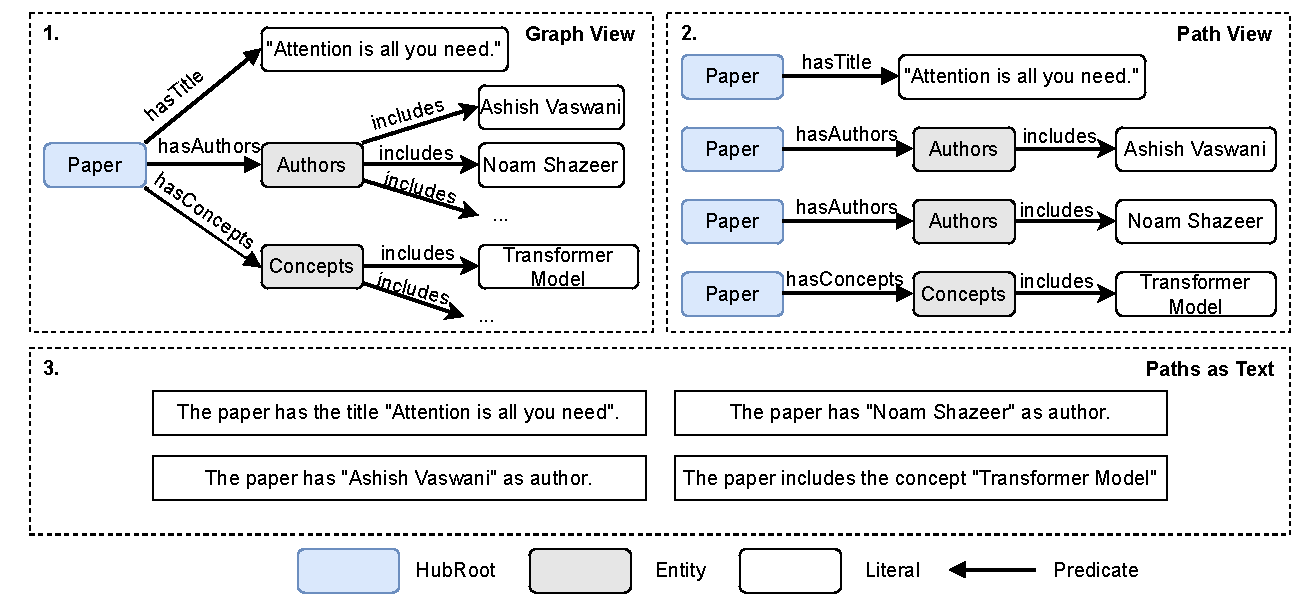
\includegraphics[width=1.0\linewidth]{figures/hublink/Hublink_figures-build_hubs.drawio.pdf}
    \caption[Path to Text Conversion]{Conversion of paths consisting of triples to textual descriptions using an \gls{llm}.}
    \label{fig:path_to_text_conversion}
\end{figure}

With the triple path $\mathcal{T}_{h_{r,i}}$, we can now define the hash value of the \texttt{HubPath} \(h_{r,i}\) as
\[
\phi_{r,i} = \text{hash}(\mathcal{T}_{h_{r,i}}) \in \mathcal{B},
\]
where \(\mathcal{B}\) is the set of all possible hash values. The hash value is generated by applying a hash function to the list of triples in the path. This will produce a unique value for each unique path, ensuring that no two paths have the same hash value, provided that the hash function is free from collisions. We then obtain the textual description of the \texttt{HubPath} \(h_{r,i}\) by applying a function:
\[
T_{\text{path}}: \mathcal{T}_{h_{r,i}} \to \mathcal{X},
\]
This function takes a triple path as input and outputs a textual description in a space \(\mathcal{X}\) of natural language strings. In \autoref{fig:path_to_text_conversion}, this process is illustrated. It shows the initial graph view and the decomposition of the hub subgraph into individual triple paths. These are then converted into a textual representation using the function \(T_{\text{path}}\) which is realized by an \gls{llm} that processes the sequence of \gls{rdf} triples $\mathcal{T}_{h_{r,i}}$ and generates a natural language description.

The final \texttt{HubPath} \(h_{r,i}\) is then defined as a tuple
\[
h_{r,i} = \bigl( \phi_{r,i}, T_{\text{path}}(\mathcal{T}_{h_{r,i}}), \mathcal{T}_{h_{r,i}} \bigr),
\]
where \(\phi_{r,i}\) is the hash value, \(T_{\text{path}}(\mathcal{T}_{h_{r,i}})\) is the textual description, and \(\mathcal{T}_{h_{r,i}}\) is the list of triples. The \texttt{HubPath} \(h_{r,i}\) is thus a representation of the path information inside a hub. This leads us to define the set of all \texttt{HubPaths} starting from the root of the hub \(r\). Formally, let \(r \in R\) be the root of the hub, where \(R\) is the set of \texttt{HubRoots} as defined in the previous section. 
We define the set of all HubPaths starting at \(r\) as
\[
\mathcal{H}(r) = \{\, h_r \mid h_r \text{ is a HubPath starting at } r \,\}.
\]

\subsection{Hub: Aggregation of Semantically Related Information}

A \texttt{Hub} is a special construct in the HubLink retriever that is used to aggregate semantically related information about a specific knowledge entity. It always consists of a \texttt{HubRoot} entity and a set of \texttt{HubPaths}. Formally, a hub is defined as
\[
Hub_r = \bigl( r,\, \mathcal{H}(r) \bigr),
\]
where \(r \in R\) is a hub root and \(\mathcal{H}(r)\) is the collection of hub paths starting from \(r\).

\subsection{HubVector: Encoding of Hub Information}
\label{sec:hublink_hubvector_definition}

To be able to efficiently retrieve relevant information from a hub, the \texttt{HubPaths} of the hub are encoded in a vector space using \texttt{HubVectors}. A \texttt{HubVector} is a low-dimensional vector representation constructed from the information of a \texttt{HubPath} and is always stored together with additional metadata that includes the hub root identifier \(r \in R\) and the textual description $T_{\text{path}}(\mathcal{T}_{h_{r,i}})$ of the \texttt{HubPath}. The goal is to project the semantic content of each \texttt{HubPath} into a vector space using a pre-trained embedding model, where a nearest-neighbor search such as \gls{ann} can be performed. What is important to consider here is that the path itself may contain too much information, which can lead to a phenomenon where the relevant information is obscured by the complexity of the path. To reduce this risk, the path is decomposed into different parts, increasing the likelihood of a nearest-neighbor search to find relevant information. More information on this design decision is provided in Section~\ref{sec:hublink_design_rationale}. 

By decomposing the \texttt{HubPath}, we define four vector representations. Let \(h_{r,i}\) denote the \(i\)-th \texttt{HubPath} of the hub with root \(r\). We define a general embedding function
\[
f: \mathcal{X} \to \mathbb{R}^d,
\]
which maps any textual input into a \(d\)-dimensional vector. We distinguish four types of \texttt{HubVectors} that can be generated from a hub path \(h_{r,i}\):

\begin{itemize}
    \item \textbf{Path Vector:} This vector represents the overall semantic content of the \texttt{HubPath}. It is obtained by embedding the full natural language description $T_{\text{path}}(\mathcal{T}_{h_{r,i}})$ of the path $\mathcal{T}_{h_{r,i}}$ generated by the \gls{llm}:
    \[
    \mathbf{v}_{\text{path}}(h_{r,i}) = f\Bigl( T_{\text{path}}(\mathcal{T}_{h_{r,i}}) \Bigr) \in \mathbb{R}^d
    \]
    
    \item \textbf{Triple Vector:} For this vector type, the triple path $\mathcal{T}_{h_{r,i}}$ is broken down into its individual triples. Each triple \(t_k \in \mathcal{T}_{h_{r,i}}\) is converted into a vector representation:
    \[
    \mathcal{V}_{\text{triples}} = \{f (t_k) \mid t_k \in \mathcal{T}_{h_{r,i}}\}, \quad f(t_k) \in \mathbb{R}^d
    \]
    
    \item \textbf{Entity Vector:} For this vector type, the triple path $\mathcal{T}_{h_{r,i}}$ is decomposed into all entities contained in the path. For each triple \(t_k = (s,p,o) \in \mathcal{T}_{h_{r,i}}\) , the entities \(s\) and \(o\) are extracted. Each entity is then embedded using \(f\):
    \[
    \mathcal{V}_{\text{entities}} = \{f(e) \mid t_k = (s, p, o) \in \mathcal{T}_{h_{r,i}},\ e \in \{s, o\}\}, \quad f(e) \in \mathbb{R}^d
    \]

    \item \textbf{Predicate Vector:} For this vector type, the hub path \(h_{r,i}\) is decomposed into all predicates contained in the path. For each triple \(t_k = (s,p,o) \in \mathcal{T}_{h_{r,i}}\), the predicate $p$ is extracted and embedded using \(f\). The embedding for each predicate is then computed as:
    \[
    \mathcal{V}_{\text{predicates}} = \{f(p) \mid t_k = (s, p, o) \in \mathcal{T}_{h_{r,i}}\}, \quad f(p) \in \mathbb{R}^d
    \]
\end{itemize}

For each hub path \(h_{r,i}\), multiple \texttt{HubVectors} are thus stored in the vector store. Each vector is stored as a tuple containing the root of the hub \(r\), the natural language description \(T_{\text{path}}(\mathcal{T}_{h_{r,i}})\), and the corresponding vector representation. Formally, we define the set of all \texttt{HubVectors} for \(h_{r,i}\) as:
\[
\begin{aligned}
    \mathcal{V}(h_{r,i}) =\;
    & \Bigl\{ \bigl( r,\; T_{\text{path}}(\mathcal{T}_{h_{r,i}}),\; \mathbf{v}_{\text{path}}(h_{r,i}) \bigr) \Bigr\} \\
    & \cup \Bigl\{ \bigl( r,\; T_{\text{path}}(\mathcal{T}_{h_{r,i}}),\; v \bigr) \mid v \in \mathcal{V}_{\text{triples}} \Bigr\} \\
    & \cup \Bigl\{ \bigl( r,\; T_{\text{path}}(\mathcal{T}_{h_{r,i}}),\; v \bigr) \mid v \in \mathcal{V}_{\text{entities}} \Bigr\} \\
    & \cup \Bigl\{ \bigl( r,\; T_{\text{path}}(\mathcal{T}_{h_{r,i}}),\; v \bigr) \mid v \in \mathcal{V}_{\text{predicates}} \Bigr\} \\
\end{aligned}
\]

Note that each vector is stored alongside the textual path description \(T_{\text{path}}(\mathcal{T}_{h_{r,i}})\) because decomposing the path into individual triples, entities, or predicates results in a loss of the semantic relationships between nodes. This can lead to reduced retrieval performance when a query matches a triple, entity, or predicate, as the isolated vector may not capture enough context to represent the full meaning. To address this, the textual description of the path \(T_{\text{path}}(\mathcal{T}_{h_{r,i}})\) is stored as metadata within each vector tuple. While the vector is used for similarity-based retrieval, the associated textual description is used during answer generation.

Finally, given a hub \(Hub_r = (r, \mathcal{H}(r))\), the overall set of \texttt{HubVectors} for the hub is defined as:
\[
\mathcal{V}(Hub_r) = \bigcup_{h \in \mathcal{H}(r)} \mathcal{V}(h).
\]
This collection of vectors, together with their associated metadata, forms the basis for the retrieval process in HubLink.



\section{Data Models}
\label{sec:hublink_data_models}

\begin{figure}
\begin{algorithmic}[1]

\Statex \textbf{Class:} \texttt{Entity} \(\leftarrow e\in E\) \Comment{Represents a node \(e\) in the graph}
    \Statex \quad ID: \texttt{String}
    \Statex \quad Value: \texttt{String}
\Statex \textbf{Class:} \texttt{Triple} \(\leftarrow  t = (s, p, o) \in G\) \Comment{Represents a triple in the graph}
    \Statex \quad Subject: \texttt{Entity}
    \Statex \quad Predicate: \texttt{String}
    \Statex \quad Object: \texttt{Entity}

\Statex
\Statex \textbf{Class:} \texttt{EntityWithDirection} \(\leftarrow (e, \text{dir}, \pi) \in \mathcal{D}_e\)
    \Statex \quad Entity: \texttt{Entity} \Comment{An entity in the graph}
    \Statex \quad Direction: \texttt{Enum} \Comment{Indicates if the entity is subject or object in the current path}
    \Statex \quad PathToEntity: \texttt{List} of \texttt{Triple} \Comment{The directed triple path leading to the entity}

\Statex
\Statex \textbf{Class:} \texttt{Hub} \(\leftarrow Hub_r = (r, \mathcal{H}(r))\)
    \Statex \quad Root: \texttt{EntityWithDirection} \Comment{The root node \(r\) of the hub}
    \Statex \quad Paths: \texttt{List} of \texttt{HubPath} \Comment{All paths in the hub rooted at \(r\)}
    \Statex \quad Score: \texttt{Float} \Comment{Combined score for all paths}

\Statex
\Statex \textbf{Class:} \texttt{HubPath} \(\leftarrow h_{r,i} \in \mathcal{H}(r)\)
    \Statex \quad PathText: \texttt{String} \Comment{Textual description of the path}
    \Statex \quad PathHash: \texttt{String} \Comment{Unique hash of the path}
    \Statex \quad Path: \texttt{List} of \texttt{Triple} \Comment{Sequence of triples representing the path}
    \Statex \quad EmbeddedText: \texttt{String} \Comment{The text used to create the embedding}
    \Statex \quad Score: \texttt{Float} \Comment{Relevance score toward the query}

\Statex
\Statex \textbf{Class:} \texttt{ProcessedQuestion}
    \Statex \quad Question: \texttt{String} \Comment{The original question that is asked}
    \Statex \quad Components: \texttt{List} of \texttt{String} \Comment{Components of the original question}
    \Statex \quad Embeddings: \texttt{List} of \texttt{List} of \texttt{Float} \Comment{Embeddings of components and question}

\Statex
\Statex \textbf{Class:} \texttt{LinkData}
    \Statex \quad HubIdentifier: \texttt{String} \Comment{Identifier associated with the data}
    \Statex \quad Text: \texttt{String} \Comment{Additional data to enrich the hub}

\end{algorithmic}
\caption[Data Models with Formal Definitions]{The data models used by HubLink mapped to their formal definitions (Data model $\leftarrow$ Formal definition).}
\label{alg:data_models}
\end{figure}


The data models used in the \textsc{HubLink} retriever are shown in \autoref{alg:data_models}. Each class corresponds to a formal element defined in Section~\ref{sec:hublink_formal_definitions}, with the mapping expressed using the notation \(\textsc{Class} \leftarrow \textsc{Formal Definition}\). In the following, we provide a description of each data model:

\paragraph{Entity} The entity data model represents a node in the graph. Each entity is associated with an identifier that uniquely identifies the entity in the graph, is associated with a value, and may also have a type. Depending on the graph, this type can be either stored directly with the entity or described using an edge to the entity. For HubLink, it is not necessary that an entity has a type, but it is advantageous for the classification of hubs.

\paragraph{Triple} The triple data model conforms to the \gls{rdf} definition. As such, it contains a subject and an object, which are both \texttt{Entity} types. The predicate describes their relation and is a \texttt{String}.

\paragraph{EntityWithDirection} This data model stores a direction and a path to an entity. Consequently, it acts as a wrapper for an \texttt{Entity} in the HubLink algorithm. 

\paragraph{Hub} The data model for a hub includes a root, which is an \texttt{EntityWithDirection} object. This root acts as a unique identifier for the hub itself and is used for building the \texttt{HubPath} objects. In addition, each hub has a score that is calculated during the retrieval to assess the relevance of the hub to the question that is asked.

\paragraph{HubPath} The data model for the \texttt{HubPath} stores the unique hash value that acts as an identifier for the \texttt{HubPath}. The textual description and the associated triple path are also stored. In addition, the model stores the text by which the path has been retrieved from the vector store. This is required as each \texttt{HubPath} is stored at different levels (path, triple, entity, or predicate level). Finally, the score that assesses the relevance of the \texttt{HubPath} to the question asked is saved in the data model.

\paragraph{ProcessedQuestion} This data model is used to store the question that is asked to the retriever, the components that have been extracted from the question, and the precomputed embeddings for both the question and the components.

\paragraph{LinkData} This data model is created during the linking process. It stores the identifier of the hub to which it is associated and a text. The text is additional information collected from an external database that is relevant to enrich the retrieval data for comprehensive answer generation.


\section{Finding Hub Root Entities}
\label{sec:hublink_finding_hub_root_entities}

\begin{algorithm}
\caption{Pseudocode for Finding Hub Root Entities}
% \caption[Pseudocode for Finding Hub Roots]{Pseudocode for finding the \texttt{HubRoot} entities of a hub. The search is performed by applying a breadth-first search where for each entity that is reached a classification takes place to classify whether this entity is qualified to be a \texttt{HubRoot}.}
\label{alg:finding_hub_roots}
\begin{algorithmic}[1]
\PersistentState
    \Statex $visited$: \texttt{Set} of \texttt{EntityWithDirection} \Comment{List of visited entities}
    \Statex $G$: \texttt{KnowledgeGraph} \Comment{The graph to search in}
\Require 
    \Statex $\vec{E}$: \texttt{List} of \texttt{EntityWithDirection} \Comment{Entities to start the search from}
    \Statex \texttt{UniformHopCount}: \texttt{Boolean} \Comment{Require uniform hop count when reaching the hubs}
\Ensure
    \Statex A tuple $(\texttt{hub\_entities}, \texttt{next\_entities})$ containing the entities that are the root of a Hub and the entities that are used to initialize the search on the next level.
\Statex
\Function{findHubRoots}{$\vec{E}, \texttt{UniformHopCount}$} 
    \State Initialize $queue \gets$ \texttt{Queue}($\vec{E}$)
    \State $hub\_roots \gets \emptyset$ \Comment{Collection of Hub root entities found}
    \State $next\_entities \gets \emptyset$ \Comment{Candidates returned for the next depth}
    
    \While{$queue \neq \emptyset$}
        \State $e \gets$ \Call{dequeue}{$queue$} \Comment{Current entity to process}
        \State \textbf{if} $e \in visited$ \textbf{then Continue}
        \State $visited \gets visited \cup \{e\}$ 
        \State $e_{\text{isHubRoot}} \gets$ \Call{isHubRoot}{$e$} \Comment{Check if entity is a hub}
        
        \If{$e_{\text{isHubRoot}}$ \textbf{and} $e \notin \text{hub\_roots}$}
            \State $hub\_roots \gets hub\_roots \cup \{e\}$
        \EndIf
        
        \If{$e_{\text{isHubRoot}}$ \textbf{and} $\neg e.\text{Left}$}
            \State \textbf{Continue} \Comment{Stop traversing the current path}
        \EndIf
        
        \State $entity\_triples \gets \{\text{All adjacent triples of } e \text{ considering its direction}\}$
        
        \If{not \texttt{UniformHopCount}}
            \State enqueue all $entity\_triples$ into $queue$
        \Else
            \State $next\_entities \gets next\_entities \cup entity\_triples$
        \EndIf
    \EndWhile
    
    \State \Return $(hub\_roots, next\_entities)$
\EndFunction

\end{algorithmic}
\end{algorithm}

The function \textsc{findHubRoots}, shown in \autoref{alg:finding_hub_roots}, is responsible for identifying the \texttt{HubRoot} entities of hubs starting from a list of input entities \(\vec{E}\), which serve as the initial traversal points within the graph \(G\). The function follows a breadth-first search strategy, meaning that all neighboring entities are explored before descending to a deeper level. To begin the search, a queue is initialized with \(\vec{E}\). Then, a loop is performed that terminates once the queue is empty. In each iteration, one entity \(e\) is dequeued and processed. If \(e\) has already been visited (as tracked in the \texttt{visited} set), it is skipped. Otherwise, it is marked as visited, and the function \texttt{isHubRoot} is called to determine whether the entity can be classified as a \texttt{HubRoot}. If \(e\) is identified as a \texttt{HubRoot} and has not already been added, it is added to the set \(hub\_roots\) to be returned once the search has finished. Next, a determination for the continuation of the search is performed. If \(e\) is a \texttt{HubRoot} and its traversal direction is \texttt{Right}, the search along that path is terminated, and the algorithm proceeds to the next entity. This is because the \texttt{HubPaths} of a hub are built following this direction, which means that those paths will be collected later during the building of the hubs. For all other cases, the function collects the triples in which \(e\) participates. These are either queued for further traversal or stored in the set \(next\_entities\), depending on the parameter \texttt{UniformHopCount}. The loop continues until the queue is empty. Once the loop ends, the function returns two sets: \(hub\_roots\), which contains the discovered hub entities, and \(next\_entities\), which are passed to the next level of traversal in the indexing process.

\begin{tcolorbox}[title=Parameter: \texttt{UniformHopCount}]
This parameter determines whether the traversal should continue beyond the first iteration and is only relevant for the \emph{graph traversal} retrieval strategy. If \(\texttt{UniformHopCount} = \texttt{False}\), all \texttt{HubRoots} directly reachable from the current entities in \(\vec{E}\) are considered. Otherwise, the traversal continues recursively until a \texttt{HubRoot} is found. This is useful when \texttt{HubRoots} lie at varying depths in the graph and a uniform number of hops to reach the entity cannot be assumed. Therefore, it should be chosen whether to set \texttt{UniformHopCount} or not based on the structure of the graph.
\end{tcolorbox}

\begin{tcolorbox}[title=Persistent State: \(\texttt{visited}\)]
The \texttt{visited} set keeps track of entities that have already been processed, taking the direction into account. This ensures that nodes are not revisited multiple times and that cycles in the graph do not cause infinite loops. Notably, this set is persistent for subsequent calls to ensure that cycles are handled for the same retrieval or indexing. Consequently, this persistent state must be cleared once the retrieval or indexing is complete, which can be accomplished by implementing the function in a class and initializing the class for each new retrieval or indexing.
\end{tcolorbox}

\begin{tcolorbox}[title=Function: \textsc{isHubRoot}]
Whether an entity is classified as a hub is determined by the \textsc{isHubRoot} function. There are several ways to do this classification, as described in Section~\ref{sec:hublink_formal_definitions}. The easiest way is to define a list of types that should be classified as a hub and check if the given entity is of that type.
\end{tcolorbox}




\section{Indexing}
\label{sec:hublink_indexing}

%%%% Algorithm for Indexing Hubs

The pseudocode for the indexing process is shown in \autoref{alg:indexing_hubs}. As input, the function requires a list of starting entities \(\vec{E}\) and the parameter \texttt{MaxIndexingDepth}, which controls how deep the algorithm traverses \(G\), and thus how large \(\hat{G}\) becomes, which is the indexed subgraph. This design choice is motivated by the potential size of the graph \(G\), which can contain millions of nodes. Using the starting entities \(\vec{E}\) and the maximum indexing depth \texttt{MaxIndexingDepth}, it allows to effectively choose between indexing the entire graph or only a subgraph \(\hat{G}\).

The indexing algorithm consists of a loop that terminates when one of the following conditions is met:
\begin{enumerate}
    \item \texttt{MaxIndexingDepth} is reached,
    \item the list of entities to process becomes empty, or
    \item no further nodes are found for traversal.
\end{enumerate}

In each iteration, the algorithm calls the function \textsc{findHubRoots} to identify \texttt{HubRoot} objects at the current depth, as well as a new set of entities to explore in the next iteration. Once found, the hub roots are passed to the \textsc{buildHubs} function, which builds the \texttt{Hub} objects. Then, to prepare the next iteration, the entities located at the ends of these hubs are added to the list of entities used to continue the indexing in the next iteration of the loop.

\begin{algorithm}[t]
\caption{Pseudocode for Indexing of Hubs}
% \caption[Pseudocode for Indexing]{Pseudocode for the indexing process. Starting from a specified set of entities, the graph is traversed up until a maximum depth while building \texttt{Hubs} for each \texttt{HubRoot} encountered during traversal.}
\label{alg:indexing_hubs}
\begin{algorithmic}[1]
\PersistentState
    \Statex $G$: \texttt{KnowledgeGraph} \Comment{The graph to search in}
\Require 
    \Statex $\vec{E}$: \texttt{List} of \texttt{Entity} \Comment{Entities from which the indexing is started}
    \Statex $\texttt{MaxIndexingDepth}$: \texttt{Integer} \Comment{Maximum allowed indexing depth}

\Procedure{hubIndexing}{$\vec{E}, \texttt{MaxIndexingDepth}$}
    \State $entities \gets \{ \texttt{EntityWithDirection}(T, \textbf{true}, \emptyset) \mid T \in \vec{E} \}$
    \State $entities \gets entities \cup \{ \texttt{EntityWithDirection}(T, \textbf{false}, \emptyset) \mid T \in \vec{E} \}$
    \If{$entities = \emptyset$}
        \State \Return
    \EndIf
    \State $depth \gets 0$ 
    
    \While{$depth \leq \texttt{MaxIndexingDepth}$}
        \State $hub\_roots, next\_entities \gets$ \Call{findHubRoots}{$entities$}
        \State $entities \gets next\_entities$
        \State $hub\_end\_entities \gets$ \Call{buildHubs}{$hub\_roots$}
        \State $entities \gets entities \cup hub\_end\_entities$
        \If{$entities = \emptyset$}
            \State \textbf{break} \Comment{Stop if no more entities to process}
        \EndIf
        \State $depth \gets depth + 1$
    \EndWhile
\EndProcedure
\end{algorithmic}
\end{algorithm}

\begin{tcolorbox}[title=Parameter: \texttt{MaxIndexingDepth}]
This parameter defines the maximum traversal depth at which \texttt{HubRoot} objects are located. It is important to note that this depth does not correspond to the entities of the graph themselves, but only those classified as \texttt{HubRoots}. Since building a hub involves traversing internal paths within the hub itself, the total depth of entities indexed may exceed \texttt{MaxIndexingDepth}.
\end{tcolorbox}




\subsection{Building Hubs}
\label{sec:hublink_building_hubs}

%%%% Algorithm for Building Hubs
\begin{algorithm}
\caption{Pseudocode for Building Hubs}
% \caption[Pseudocode for Building Hubs]{Pseudocode for building \texttt{Hub} objects. This involves an update check to determine, whether the hub needs to be updated or the current index is already up-to-date. The function then creates the \texttt{HubPath} objects of the hub and stores them in the vector store.}
\label{alg:building_hubs}
\begin{algorithmic}[1]
\PersistentState
    \Statex $\hat{V}$: \texttt{VectorStore} \Comment{Persistent storage for hub-related data}
\Require 
    \Statex $\vec{R}$: \texttt{List} of \texttt{Entity} \Comment{Root entities of the hubs}
\Ensure
    \Statex A list of entities that are used for the next indexing depth.

\Statex
\Function{buildHubs}{$\vec{R}$}
    \State $next\_entities \gets \emptyset$ \Comment{Entities for deeper indexing}
    \ForAll{$r \in \vec{R}$}
        \State $(\vec{p}, \vec{e}) \gets$ \Call{findPathsInHub}{$r$}
        \State $next\_entities \gets next\_entities \cup \vec{e}$
        
        \State $needs\_rebuild \gets$ \Call{hubIndexNeedsToBeUpdated}{$r, \vec{p}$}
        
        \If{$needs\_rebuild$}
            \State $hub\_paths \gets$ \Call{buildHubPaths}{$\vec{p}$}
            \State \Call{storeHubPaths}{$hub\_paths, r$}
        \EndIf
    
    \EndFor
    \State \Return $next\_entities$
\EndFunction
\end{algorithmic}
\end{algorithm}

A hub $Hub_r \bigl(r, \mathcal{H}(r) \bigr)$ consists of the root $r$ and the \texttt{HubPaths} $\mathcal{H}(r)$. Consequently, the building process is two-fold. First, the triple paths of a hub have to be extracted from the graph, and then the \texttt{HubPath} objects have to be created. Then, the paths have to be stored in the vector store.

The function for building hubs is detailed in \autoref{alg:building_hubs}. This function takes as input a list of root entities \(\vec{R}\), each of which is assumed to be confirmed \texttt{HubRoot} objects. The algorithm then iterates over every entity \(r \in \vec{R}\) to construct the corresponding hub. This is realized in a loop that processes each root entity \(r\). It calls the function \textsc{findPathsInHub} that identifies and returns all triple paths originating from \(r\) that are relevant for building the \texttt{HubPath} objects. The function further returns a set of additional entities that may serve as roots for nested hubs, which are collected in the set \(next\_entities\) for further indexing. Next, the function \textsc{hubIndexNeedsToBeUpdated} is invoked to determine whether the current hub must be created or updated. If this is the case, \textsc{buildHubPaths} is called to generate a new set of \texttt{HubPath} objects based on previously identified paths. After the paths have been collected, the \textsc{storeHubPaths} function is called, which adds them to the vector store.

\begin{tcolorbox}[title=Persistent Storage: Vector Store \(\hat{V}\)]
The vector store \(\hat{V}\) serves as persistent storage for all indexed \texttt{HubPath} objects. As mentioned in Section~\ref{sec:hublink_formal_definitions}, it stores four types of vectors on the path, triple, entity, and predicate level. During indexing, the vector store is filled with the vectors, and during retrieval, similarity matches to the vectors are performed to find those \texttt{HubPath} objects that are most relevant to the query.
\end{tcolorbox}

\subsection{Checking for Graph Updates}

\begin{algorithm}
\caption{Pseudocode for Determining Index Update}
% \caption[Pseudocode for Determining Index Update]{Pseudocode for checking whether the index of a \texttt{Hub} needs to be updated. This is done by verifying whether all \texttt{HubPaths} include the same content as the graph.}
\label{alg:hub_update_check}
\begin{algorithmic}[1]
\PersistentState
    \Statex $\hat{V}$: \texttt{VectorStore} \Comment{A vector store to store hub data}
\Require 
    \Statex $r$: \texttt{EntityWithDirection} \Comment{The root entity of the hub}
    \Statex $\vec{p}$: \texttt{List} of \texttt{List} of \texttt{Triple} \Comment{The collected paths for the hub}
\Ensure
    \Statex \texttt{Boolean} indicating whether the hub data in the vector store needs to be updated

\Statex
\Function{hubIndexNeedsToBeUpdated}{$r, \vec{p}$}
    \State $\delta \gets$ \Call{computeHashesForPaths}{$\vec{p}$}
    \State $\gamma \gets$ \Call{getStoredPathHashes}{$r$}
    \If{$\delta \neq \gamma$}
        \State \Return \textbf{true}
    \Else
        \State \Return \textbf{false}
    \EndIf
\EndFunction
\Statex
\Function{getStoredPathHashes}{$r$}
    \State $v \gets \hat{V}.\Call{getAllPathVectors}{r}$
    \State $\gamma \gets \emptyset$
    \ForAll{$vector \in v$}
        \State $h \gets vector.metadata.pathHash$
        \State $\gamma \gets \gamma \cup \{h\}$
    \EndFor
    \State \Return $\gamma$
\EndFunction
\Statex
\Function{computeHashesForPaths}{$\vec{p}$}
    \State $\delta \gets \emptyset$
    \ForAll{$p \in \vec{p}$}
        \State $\delta \gets \delta \cup \{\Call{hash}{p}\}$
    \EndFor
    \State \Return $\delta$
\EndFunction
\end{algorithmic}
\end{algorithm}

\autoref{alg:hub_update_check} provides pseudocode to verify whether the index of a hub stored in the vector store \(\hat{V}\) is still consistent with the current state of the graph. It plays a key role in ensuring that the index remains consistent with the underlying graph without unnecessarily rebuilding hubs that are already up-to-date. 

The check is performed by the function \textsc{hubIndexNeedsToBeUpdated}, which takes as input the root entity \(r\) of a hub and a list of current triple paths \(\vec{p}\). The function operates under the assumption that the paths in \(\vec{p}\) represent the latest structure of the graph. To verify consistency, it first computes a hash value for each triple path and stores the resulting set in \(\delta\) via the function \textsc{computeHashesForPaths}. These hashes serve as a signature of the current hub structure. Next, the function \textsc{getStoredPathHashes} retrieves the stored path hashes from the vector store \(\hat{V}\) for the given root entity \(r\). These are collected in the set \(\gamma\), which represents the last known indexed state of the hub. Finally, the sets \(\delta\) and \(\gamma\) are compared. If they differ, it means that the indexed hub is outdated and needs to be rebuilt. In this case, the function returns \texttt{true}. Otherwise, it returns \texttt{false}.

Using hash values to compare hub path structures offers an efficient and scalable way to detect changes without needing to perform expensive graph diffing or structural comparisons. Each triple path is mapped to a compact, fixed-size hash, which acts as a unique signature of its content. This allows the algorithm to perform fast set-based comparisons between the current state of the graph and the previously stored hub data. As long as the hash function is consistent and resistant to collision, this approach reliably identifies when any part of the path structure of a hub has changed, thus triggering a rebuild only when necessary.


\subsection{Finding the Triple Paths of a Hub}

\begin{algorithm}[p]
\caption{Pseudocode for Finding the Triple Paths of a Hub}
% \caption[Pseudocode for Finding the Hub Triple Paths]{Pseudocode for finding the paths consisting of triples with a \texttt{HubRoot} entity as the root of each path.}
\label{alg:finding_paths_in_hub}
\begin{algorithmic}[1]
\PersistentState
    \Statex $G$: \texttt{KnowledgeGraph} \Comment{The graph to search in}
\Require 
    \Statex $R$: \texttt{Entity} \Comment{Root entity of the hub}
    \Statex \texttt{MaximumPathLength}: \texttt{Integer} \Comment{Maximum allowed path length}
\Ensure
    \Statex A tuple \((paths, candidates)\), where $paths$ are the collected triple paths, and $candidates$ are entities at hub boundaries

\Statex
\Function{findPathsInHub}{$R, \texttt{MaximumPathLength}$}
    \State $visited \gets \emptyset$ \Comment{Set of entities visited}
    \State $candidates \gets \emptyset$ \Comment{Candidates for next level}
    \State $paths \gets \emptyset$ \Comment{Paths of triples from the graph}
    \State $queue \gets$ a new queue initialized with \((R, \emptyset)\)
    
    \While{$queue \neq \emptyset$}
        \State $(e, \vec{p}) \gets$ \Call{dequeue}{$queue$} \Comment{Current entity and path}
        \If{$e \in visited$ and $e \neq R$}
            \State \textbf{continue} \Comment{Avoid revisiting entities}
        \EndIf
        \State $visited \gets visited \cup \{e\}$

        \If{$|\vec{p}| \geq \texttt{MaximumPathLength}$}
            \State $paths \gets paths \cup \{\vec{p}\}$
            \State \textbf{continue}
        \EndIf
        
        \State $\vec{t} \gets$ \Call{getOutboundTriples}{$e, G$} \Comment{Retrieve all neighbors of $e$}
        \If{$\vec{t} = \emptyset$}
             \State $paths \gets paths \cup \{\vec{p}\}$ \Comment{Leaf entity of graph reached}
            \State\textbf{continue}
        \EndIf
        
        \ForAll{$triple \in \vec{t}$}
            \State $e' \gets triple.Object$
            \If{$e' = R$}
                \State \textbf{continue} \Comment{Skip cycles back to root}
            \EndIf
            \If{\Call{isHubRoot}{$e'$}}
                \State $candidates \gets candidates \cup \{e'\}$
                \State $paths \gets paths \cup \{\vec{p}\}$
            \Else
                \State $\vec{p'} \gets \vec{p} \mathbin{++} \{triple\}$ \Comment{Append triple to path}
                \State enqueue \((e', \vec{p'})\) into $queue$ \Comment{Add neighbor to queue}
            \EndIf
        \EndFor
    \EndWhile
    
    \State \Return $(paths, candidates)$
\EndFunction
\end{algorithmic}
\end{algorithm}

To find all relevant triple paths associated with a hub, the function \textsc{findPathsInHub}, shown in \autoref{alg:finding_paths_in_hub}, is used. This function is invoked with the root entity \(R\) of a hub, the knowledge graph \(G\), and the parameter \(\texttt{MaximumPathLength}\). It returns all valid triple paths starting at \(R\), together with a list of candidate entities that mark the boundary of the hub for further indexing.

At the start of the function, three sets are initialized: \texttt{visited}, \texttt{candidates}, and \texttt{paths}. The \texttt{visited} set tracks entities already explored to prevent cycles. The \texttt{candidates} set stores entities that are themselves hubs and may serve as roots for nested hubs in later indexing stages and the \texttt{paths} set contains all complete triple paths discovered within the hub.

A queue is initialized with a tuple containing the root entity \(R\) and an empty path. The function performs a breadth-first traversal using this queue. In each iteration, an entity \(e\) and its associated path \(\vec{p}\) are dequeued. If \(e\) has already been visited and is not the root, it is skipped. If the current path length has reached the maximum allowed length, the path is stored, and traversal for that branch ends. Otherwise, the function retrieves all outbound triples of \(e\). If there are no outbound triples, the node is considered a leaf, and the current path is saved. However, if there are outbound triples, each triple is examined. This is done by extracting the entity object \(e'\) from the triple. The reason we are only looking at the objects of the \gls{rdf} triples is that, by convention, the paths of a hub are only examined in the natural direction of the graph. The algorithm then continues by checking whether \(e'\) is the \texttt{HubRoot} of the hub \(R\). In this case, it is skipped to avoid cycles. If \(e'\) is identified as a \texttt{HubRoot} for another hub, it is added to the \texttt{candidates} set, and the current path is stored without traversing further in that direction. Otherwise, the triple is appended to the current path and the new state \((e', \vec{p}')\) is enqueued for further exploration. This process continues until the queue is empty. At that point, all discovered paths and candidate hub boundaries have been collected and are returned by the function.

\begin{tcolorbox}[title=Parameter: \texttt{MaximumPathLength}]
The parameter \texttt{MaximumPathLength} limits how deeply the algorithm explores the graph from the \texttt{HubRoot} $R$. It defines the maximum allowed length of any \texttt{HubPath} and helps control the scope and relevance of each path. A path that is too long may lose semantic connection to the core context of the hub. Therefore, choosing an appropriate value for \texttt{MaximumPathLength} depends on the structure and density of the graph.
\end{tcolorbox}



\begin{algorithm}[ht]
\caption{Pseudocode for Building HubPaths}
% \caption[Pseudocode for Building HubPaths]{Pseudocode for building \texttt{HubPath} objects. Based on the given triple paths, a unique hash value and a textual description is generated for which each \texttt{HubPath} is initialized and then returned.}
\label{alg:building_hub_paths}
\begin{algorithmic}[1]
\Require 
    \Statex $\vec{T}$: \texttt{List} of \texttt{List} of \texttt{Triple} \Comment{The paths to process}
\Ensure
    \Statex A list of \texttt{HubPath} objects.

\Statex
\Function{buildHubPaths}{$\vec{T}$}
    \State $hub\_paths \gets \emptyset$
    
    \ForAll{$\vec{t} \in \vec{T}$}
        \State $\delta \gets$ \Call{hash}{$\vec{t}$} \Comment{Calculate unique path identifier}
        \State $\mathcal{T} \gets$ \Call{pathToText}{$\vec{t}$}
        \State $hub\_paths \gets hub\_paths \cup \{\texttt{HubPath}(\mathcal{T}, \delta, \vec{t})\}$
    \EndFor
    \State \Return $hub\_paths$
\EndFunction      
\Statex
\Function{pathToText}{$\vec{t}$}
    \State \Return Convert $\vec{t}$ to text using an LLM
\EndFunction
\end{algorithmic}
\end{algorithm}

\subsection{Building the HubPaths of a Hub}

As defined in Section~\ref{sec:hublink_formal_definitions}, a \texttt{HubPath} consists of a hash value, a natural language description, and a path of triples. The function \textsc{buildHubPaths}, shown in \autoref{alg:building_hub_paths}, is responsible for generating the \texttt{HubPath} objects associated with a hub. It takes as input a list \(\vec{T}\), where each element \(\vec{t} \in \vec{T}\) is a path composed of \gls{rdf} triples originating from the root. For each path \(\vec{t}\), a unique identifier \(\delta\) is computed by hashing the content of the path. This hash serves as an identifier for identifying the \texttt{HubPath} object. The path is then converted into a textual representation \(\mathcal{T}\) using the function \textsc{pathToText}, which uses an \gls{llm} to generate a natural language description of the path. The resulting \texttt{HubPath} object is then instantiated using the hash \(\delta\), the textual description \(\mathcal{T}\), and the original triple path \(\vec{t}\). All such \texttt{HubPath} objects are collected and returned as the output of the function.



\subsection{Storing the HubPath Objects}

\begin{algorithm}
\caption{Pseudocode for Storing HubPaths in the Vector Store}
% \caption{Pseudocode for storing the vectors of \texttt{HubPath} objects. There are four types of vectors that are stored in the vector store which are on the path, triple, entity, or predicate level. Each vector is stored with metadata to identify the associated \texttt{HubPath} of the vector.}
\label{alg:storing_vectors}
\begin{algorithmic}[1]
\PersistentState
    \Statex $\hat{V}$: \texttt{VectorStore} \Comment{A vector store to store hub data}
\Require
    \Statex $\vec{H}$: List of \texttt{HubPath} \Comment{Hubpath objects to store in the vector store}
    \Statex $r$: \texttt{HubRoot} \Comment{Root entity of the hub the paths are associated with}

\Procedure{storeHubPaths}{$\vec{H}, r$}
    \State $\hat{V}$.\Call{deleteHubPaths}{$r$} \Comment{Delete existing paths of the root entity $r$}
    \ForAll{$h \in \vec{H}$}
        \State $metadata \gets (r, h.PathHash, h.PathText, h.Path)$ \Comment{Metadata for the vectors}
        \State \Call{storePath}{$h.PathText$, $metadata$} \Comment{Store the path vector}
        \State \Call{storeTriples}{$h.Path, metadata$} \Comment{Store the triples in the vector store}
        \State \Call{storeEntities}{$h.Path, metadata$} \Comment{Store the entities in the vector store}
        \State \Call{storePredicates}{$h.Path, metadata$} \Comment{Store the predicates in the vector store}
    \EndFor
\EndProcedure

\Statex
\Procedure{storePath}{$\mathcal{T}$, $metadata$}
    \State \Call{addToVectorStore}{$\mathcal{T}, metadata$}
\EndProcedure

\Statex
\Procedure{storeTriples}{$\vec{t}, metadata$}
     \ForAll{$triple \in \vec{t}$} 
        \State \Call{addToVectorStore}{$triple.subject, metadata$} 
    \EndFor
\EndProcedure

\Statex
\Procedure{storeEntities}{$\vec{t}, metadata$}
    \State $entities \gets \emptyset$ 
    \ForAll{$triple \in \vec{t}$}
        \State $entities \gets entities \cup \{triple.subject\}$
        \State $entities \gets entities \cup \{triple.object\}$ 
    \EndFor
    \ForAll{$e \in entities$} 
        \State \Call{addToVectorStore}{$e, metadata$} 
    \EndFor
\EndProcedure

\Statex
\Procedure{storePredicates}{$\vec{t}, metadata$}
    \State $predicates \gets \emptyset$ 
    \ForAll{$t \in \vec{t}$} 
        \State $predicates \gets predicates \cup \{t.predicate\}$
    \EndFor
    \ForAll{$p \in predicates$} 
        \State \Call{addToVectorStore}{$p, metadata$} 
    \EndFor
\EndProcedure
\Statex
\Procedure{addToVectorStore}{$itemToEmbed, metadata$}
    \State $\vec{\mu} \gets$ \Call{getEmbedding}{$itemToEmbed$} \Comment{Embed the text}
    \State $\delta \gets$ \Call{hash}{$object$} \Comment{Hash the text to get a unique key}
    \State $etadata \gets metadata \mathbin{++} itemToEmbed$ \Comment{Add embedded text to metadata}
    \State $\hat{v}$.\Call{store}{$\delta$, $\vec{\mu}$, $metadata$} \Comment{Add the vector by key with the metadata}
\EndProcedure
\end{algorithmic}
\end{algorithm}

\autoref{alg:storing_vectors} presents the pseudocode of the \textsc{storeHubPaths} function, which stores \texttt{HubPath} objects in the vector store \(\hat{V}\). The function takes as input a list of \texttt{HubPath} objects and a \texttt{HubRoot} entity $r$. It first deletes any previously stored \texttt{HubPath} objects associated with \(r\) from the vector store \(\hat{V}\) to ensure that outdated representations do not persist across indexing runs. Then, for each \texttt{HubPath} \(h\), the function prepares metadata, including the root entity, a path hash, a natural language description, and the triple path itself. This metadata is then used in a series of helper functions, each responsible for storing a specific vector type, as defined in Section~\ref{sec:hublink_formal_definitions}.

There are various helper functions involved for storing the \texttt{HubPath} at different vector levels. The helper function is \textsc{addToVectorStore} which is used by all the subsequent storing methods. This function receives as input any text to then embed it into a vector, creates a hash value that acts as a unique key, and stores the embedding with the metadata at the location in the vector store associated with the key. The following helper functions are used for storing the \texttt{HubPath} at different vector levels. First, \textsc{storePath} stores the textual description of the \texttt{HubPath}. Then, the function \textsc{storeTriples} extracts all triples from the path and stores each one separately. Next, \textsc{storeEntities} collects all subjects and objects from the triples and \textsc{storePredicates} extracts all predicates.

\begin{tcolorbox}[title=Path Hash: Unique Vector Key]
Hashing the path to a unique key allows efficient storage and updating of vector entries in the vector store. Because the hash depends on the content of the path, any structural change will result in a different hash. This ensures that updates to paths can be recognized during an update of the index without having to recalculate the entire index.
\end{tcolorbox}


\section{Vector Store Retrieval}
\label{sec:hublink_vector_store_operations}

During the indexing process, the \texttt{HubPath} objects of a \texttt{Hub} have been stored in a vector store. This section details the algorithms for retrieving these \texttt{HubPath} objects. Specifically, we first outline the procedures for their retrieval from the vector store before explaining the diversity-based ranking algorithm applied to diversify the retrieval.

\subsection{Global Retrieval of HubPaths}

\begin{algorithm}[t]
\caption{Pseudocode for Global HubPath Retrieval}
% \caption[Pseudocode for Global HubPath Retrieval]{Pseudocode for retrieving relevant hubs using a global similarity search. During this search, the embeddings from the question and its components are used to do a global nearest-neighbor search on the vector store to find the most related \texttt{HubPath} objects.}
\label{alg:global_similarity_search}
\begin{algorithmic}[1]
\PersistentState
    \Statex $\hat{V}$: \texttt{VectorStore} \Comment{Stores all vector representations for hub paths}
\Require 
    \Statex $\hat{Q}$: \texttt{ProcessedQuestion} \Comment{The processed question}
    \Statex $\vec{H}$: \texttt{List} of \texttt{Hub} \Comment{Hubs excluded from the search}
    \Statex \texttt{TopPathsToKeep}: \texttt{Integer} \Comment{Number of paths considered for each Hub}
\Ensure
    \Statex A list of \texttt{Hub} objects most relevant to the question

\Function{globalSimilaritySearch}{$\hat{Q}, \vec{H}, \texttt{TopPathsToKeep}$}
    \State $excluded \gets \{h.Root \mid h \in \vec{H}\}$ \Comment{Hubs excluded from the search}
    \State $filter \gets \texttt{hub\_entity} \notin excluded$ \Comment{Filter for the vector store query}
    \State $n\_results \gets \texttt{TopPathsToKeep} \cdot 2$ \Comment{Number of hub paths to return}
    \State $\vec{\mu} \gets \emptyset$ \Comment{Set of unique path hashes}

    \While{$|\vec{\mu}| < n\_results$}
        \State $\vec{\phi} \gets \hat{V}$.\Call{query}{$\hat{Q}.Embeddings, n\_results, filter$}
    
        \If{$\vec{\phi} = \emptyset$}
            \State \textbf{break}
        \EndIf
        
        \State $paths \gets$ empty map from \texttt{Entity} to \texttt{List} of \texttt{HubPath}
        
        \ForAll{$\phi \in \vec{\phi}$}
            \State $hub\_path \gets$ \Call{convertToHubPath}{$\phi$} \Comment{Convert result to HubPath object}
            \If{$hub\_path.PathHash \in \vec{\mu}$}
                \State \textbf{continue} \Comment{Skip duplicate paths}
            \EndIf
            \State $hub\_entity \gets \phi.metadata.RootEntity$
            \State $paths[hub\_entity] \gets paths[hub\_entity] \cup \{hub\_path\}$
            \State $\vec{\mu} \gets \vec{\mu} \cup \{hub\_path.PathHash\}$
        \EndFor
    \EndWhile
    
    \State $final\_hubs \gets \emptyset$

    \ForAll{$(root, paths) \in paths$}
        \State $ranked \gets$ \Call{applySubjectDiversityRanker}{$paths$}
        \State $pruned \gets$ \Call{prunePaths}{$ranked$, \texttt{TopPathsToKeep}}
        \State $hub \gets$ \texttt{Hub}$(root, pruned)$
        \State $final\_hubs \gets final\_hubs \cup \{hub\}$
    \EndFor

    \State \Return $final\_hubs$ \Comment{Return the ranked hubs}

\EndFunction

\end{algorithmic}
\end{algorithm}

The function \textsc{globalSimilaritySearch}, shown in \autoref{alg:global_similarity_search}, is responsible for retrieving the most relevant hubs from the vector store \(\hat{V}\) based on a given question. It takes as input a \texttt{ProcessedQuestion} object \(\hat{Q}\), a list of \texttt{Hub} objects to exclude \(\vec{H}\), and the number of top paths to keep per hub, specified by the parameter \texttt{TopPathsToKeep}.

The function starts by constructing a filter to exclude all root entities of the hubs already contained in \(\vec{H}\). Then, it proceeds with an iterative loop. The loop starts by querying the vector store with the embeddings of \(\hat{Q}\), asking for the \(2 \cdot \texttt{TopPathsToKeep}\) most similar vectors that conform to the filter. This search is an \gls{ann} search that ranks the results according to the similarity of the question vector with the vectors stored in the database. The reason we are multiplying the number of retrieved paths by two is to ensure a sufficient candidate pool for the following diversity-based ranking. If no results are returned for the query, the loop is terminated early. Otherwise, it initializes a mapping called \texttt{paths}, which groups retrieved paths by their associated hub entities. Each result \(\phi\) is processed by extracting the root of the hub from the metadata and converting the vector representation into a \texttt{HubPath} object. Subsequent to the conversion process, a verification procedure is initiated to determine whether the specified path has been previously added. This verification is conducted by comparing the hash value of the given path with those stored in a list of unique hash values. In the event that the path has not been previously added, it is appended to the map at the entry of its root. Following this, the loop progresses if not enough paths have been extracted from the vector store. Otherwise, the loop is terminated.

Afterwards, the function initializes an empty list called \texttt{final\_hubs}, which is later returned. For each hub root entity in \texttt{paths}, the associated paths are passed to the function \textsc{applySubjectDiversityRanker} (see Section~\ref{sec:hublink_pseudocode_diversity_ranker}), which ranks them by semantic relevance while promoting subject diversity at the triple level. The ranked list is then pruned to retain only the top \texttt{TopPathsToKeep} paths. Finally, a new \texttt{Hub} object is created for each root entity using the ranked and pruned paths, and the resulting hubs are collected in \texttt{final\_hubs}. Once all candidates are processed, the list of hubs is returned.


\subsection{Hub-Specific HubPath Retrieval}

\begin{algorithm}[t]
\caption{Pseudocode for HubPath Retrieval}
% \caption{Pseudocode for retrieving the \texttt{HubPath} objects of a hub. The search is done using a nearest-neighbor search on the vector store using the embeddings of the question and its components to find the most related \texttt{HubPath} objects that are associated with a specific \texttt{HubRoot}}
\label{alg:get_hub_paths_for_hub}
\begin{algorithmic}[1]
\PersistentState
    \Statex $\hat{V}$: \texttt{VectorStore} \Comment{Stores all vector representations for hub paths}
\Require 
    \Statex $r$: \texttt{Entity} \Comment{The root entity of the hub}
    \Statex $\hat{Q}$: \texttt{ProcessedQuestion} \Comment{The processed question}
    \Statex \texttt{TopPathsToKeep}: \texttt{Integer} \Comment{Number of paths to keep for this hub}
\Ensure
    \Statex A list of \texttt{HubPath} objects associated with root entity $r$

\Function{getHubPathsForHub}{$r, \hat{Q}, \texttt{TopPathsToKeep}$}
    \State $\vec{\mu} \gets \emptyset$ \Comment{Set of unique path hashes}
    \State $hub\_paths \gets \emptyset$ \Comment{List of HubPaths to return}

    \While{$|\vec{\mu}| < \texttt{TopPathsToKeep}$}
        \State $filter \gets \{\texttt{path\_hash} \notin \vec{\mu} \land \texttt{hub\_entity} = r\}$
        \State $n\_results \gets \texttt{TopPathsToKeep} \cdot 2$
        \State $\vec{r} \gets \hat{V}$.\Call{query}{$\hat{Q}.Embeddings, n\_results, filter$}

        \If{$\vec{r} = \emptyset$}
            \State \textbf{break} \Comment{No more paths to process}
        \EndIf

        \State $parsed\_paths \gets$ \Call{convertToHubPaths}{$\vec{r}$} \Comment{Convert results to HubPath objects}
        
        \State $ranked\_paths \gets$ \Call{applySubjectDiversityRanker}{$parsed\_paths$}

       \ForAll{$hub\_path \in ranked\_paths$}
            \If{$hub\_path.PathHash \in \vec{\mu}$}
                \State \textbf{continue} \Comment{Skip duplicate paths}
            \EndIf

            \If{$|hub\_paths| \geq \texttt{TopPathsToKeep}$}
                \State \textbf{break} \Comment{Reached the limit of paths to keep}
            \EndIf

            \State $hub\_paths \gets hub\_paths \cup \{hub\_path\}$
            \State $\vec{\mu} \gets \vec{\mu} \cup \{hub\_path.PathHash\}$
        \EndFor
    \EndWhile
    
    \State \Return $hub\_paths$
\EndFunction
\end{algorithmic}
\end{algorithm}

\autoref{alg:get_hub_paths_for_hub} presents the pseudocode for retrieving the top \texttt{TopPathsToKeep} hub paths associated with a specific root entity \(r\). The \textsc{getHubPathsForHub} function takes as input the root entity \(r\), a processed question \(\hat{Q}\), and the number of paths to retain. The output is a ranked and pruned list of \texttt{HubPath} objects that are most relevant to the question.

First, the function initializes two collections: \(\vec{\mu}\) and \texttt{hub\_paths}. The former stores the hash values of the already selected paths and the latter stores the actual \texttt{HubPath} objects to return. The main loop continues until the number of unique paths collected in \(\vec{\mu}\) reaches the desired count, \texttt{TopPathsToKeep}. In each iteration, a filter is constructed to exclude already seen path hashes and to restrict the search to paths associated with the current hub entity \(r\). The vector store \(\hat{V}\) is then queried for up to \(2 \cdot \texttt{TopPathsToKeep}\) results matching this filter. This over-retrieval is intentional as it provides a larger candidate pool for the \textsc{applySubjectDiversityRanker} (see Section~\ref{sec:hublink_pseudocode_diversity_ranker}), which reranks the results to promote subject diversity among the selected paths. If the query returns no results, the loop terminates. Otherwise, the results are converted into \texttt{HubPath} objects and passed to the diversity ranker. The ranked paths are then iterated over. If the hash of a path already exists in \(\vec{\mu}\), it is skipped to avoid duplicates. This is necessary because each \texttt{HubPath} is stored at multiple representation levels in the vector store (see Section~\ref{sec:hublink_hubvector_definition}), and this process ensures that only the version of each path with the highest initial similarity score remains, thereby ensuring relevance. If the number of retained paths reaches \texttt{TopPathsToKeep}, the loop exits early. Otherwise, the current path is added to \texttt{hub\_paths}, and its hash is added to \(\vec{\mu}\). If too many duplicates were encountered in the current iteration, this could lead to a situation where the number of unique paths has not yet reached the desired number. In this case, the loop continues, using the updated filter to retrieve more candidates. Once the loop terminates, the function returns the final list of \texttt{HubPath} objects associated with root \(r\) that are most relevant to the question.



\subsection{Diversity-Based Ranking of HubPaths}
\label{sec:hublink_pseudocode_diversity_ranker}

\begin{algorithm}[t]
\caption{Pseudocode for Diversity Ranking of HubPaths}
% \caption{Pseudocode for reranking \texttt{HubPath} objects by penalizing repeated subjects to promote semantic diversity.}
\label{alg:diversity_ranking}
\begin{algorithmic}[1]
\Require 
    \Statex $\vec{h}$: \texttt{List} of \texttt{HubPath} \Comment{HubPaths to rerank}
    \Statex \texttt{DiversityPenalty}: \texttt{Float} \Comment{Penalty applied for repeated subjects}
\Ensure
    \Statex A reranked list of \texttt{HubPath} objects promoting subject diversity

\Function{applySubjectDiversityRanker}{$\vec{h}, \texttt{DiversityPenalty}$}
    \State $pre\_sorted \gets$ \Call{sortByScore}{$\vec{h}$} \Comment{Initial sort by original score}

    \State $subject\_counts \gets$ empty map from subject to count

    \ForAll{$h \in pre\_sorted$}
        \State $text \gets h.EmbeddedText$
        \State $subject \gets$ \Call{extractSubject}{$text$} \Comment{Extract the subject from the text}
        \If{$subject \neq$ \texttt{None}}
            \State $count \gets$ \Call{getOrDefault}{$subject\_counts$, $subject$, $0$}
            \State $h.Score \gets h.Score - (\texttt{DiversityPenalty} \cdot count)$
            \State $subject\_counts[subject] \gets count + 1$
        \EndIf
    \EndFor
        
    \State $reranked \gets$ \Call{sortByScore}{$\vec{h}$} \Comment{Re-sort by adjusted scores}
    \State \Return $reranked$

\EndFunction
\end{algorithmic}
\end{algorithm}

The pseudocode for the function \textsc{applySubjectDiversityRanker} is shown in \autoref{alg:diversity_ranking}. The goal of this function is to promote diversity among the retrieved \texttt{HubPath} objects by penalizing paths that share the same subject entity. This is particularly useful in cases where multiple paths are relevant but semantically redundant due to overlapping subjects. The rationale behind this reranking approach is discussed in more detail in Section~\ref{sec:hublink_design_rationale}.

The function takes as input a list of \texttt{HubPath} objects \(\vec{h}\) and a diversity penalty parameter \texttt{DiversityPenalty}. It begins by sorting the paths in descending order on the basis of their initial scores. Next, the function initializes a subject frequency map \texttt{subject\_counts}, which tracks how many times each subject appears across the paths. The algorithm then iterates through the sorted list of \texttt{HubPath} objects. For each path \(h\), the subject is extracted from the text that was used to embed the path using the function \textsc{extractSubject}. However, this extraction only returns a subject if the text that was embedded actually represents a triple. The reason why the text may not be a triple comes from the different content levels at which the \texttt{HubPaths} are embedded, which are path, triple, entity, or predicate, as explained in Section~\ref{sec:hublink_formal_definitions}. If a subject is successfully extracted from the text, a penalty is applied to the score of the path based on how often that subject has previously appeared. Specifically, the score is reduced by the product of \texttt{DiversityPenalty} and the current count for that subject. After applying the penalty, the count of the extracted subject is incremented in \texttt{subject\_counts}, ensuring that repeated appearances of the same subject are penalized more heavily on subsequent occurrences. Finally, the function applies a second sorting on the modified list of paths and returns the result. 


\section{Retrieval}
\label{sec:hublink_retrieval_strategies}

The following section describes the retrieval process of the HubLink retriever. This process is responsible for finding the hubs and their associated paths that can be used to generate partial answers that are then consolidated into a final answer. Two strategies for retrieval are proposed. The \emph{Direct Retrieval Strategy} offers faster retrieval with reduced accuracy for local queries, whereas the \emph{Graph Traversal Strategy} improves local query precision but requires more execution time. Both strategies receive a \texttt{ProcessedQuestion} object as input, the explanation of which we are going to start in the following.

\subsection{Question Processing}

\begin{algorithm}[t]
\caption{Pseudocode for Creating a ProcessedQuestion}
% \caption{Pseudocode for creating a \texttt{ProcessedQuestion} object. This object contains the original question and its embedding as well as the semantic components, extracted using an \gls{llm} from the question and their embeddings.}
\label{alg:question_processing}
\begin{algorithmic}[1]
    \Require 
        \Statex $Q$: \texttt{String} \Comment{The question being asked}
    \Ensure
        \Statex A \texttt{ProcessedQuestion} object containing embeddings and components

    \Function{processQuestion}{$Q$}
        \State $embeddings \gets \emptyset$
        \State $q\_embedding \gets$ \Call{getEmbedding}{$Q$} \Comment{Embed the question}
        \State $embeddings \gets embeddings \cup \{q\_embedding\}$

        \State $components \gets$ \Call{extractComponents}{$Q$}
        \ForAll{$c \in components$}
            \State $embeddings \gets embeddings \cup \{\Call{getEmbedding}{c}\}$
        \EndFor

        \State \Return $\texttt{ProcessedQuestion}(Q, components, embeddings)$
    \EndFunction

    \Statex
    \Function{extractComponents}{$Q$}
        \State \Return Extract components from $Q$ using an LLM
    \EndFunction
\end{algorithmic}
\end{algorithm}

The first step in the retrieval process is to preprocess the question \(Q\). This involves two tasks: extracting the semantic components of the question and computing vector embeddings for both the question and the components of the question using an embedding model. This procedure is illustrated in the pseudocode in \autoref{alg:question_processing}, which defines the function \textsc{processQuestion}. 

The function receives the question as input and starts by computing an embedding of the entire question using a pre-trained embedding model. Next, the semantic components are extracted from the question using an \gls{llm}. By identifying individual components such as entities, types, time expressions, or contextual constraints, the retriever can perform more granular matching during the retrieval phase. This step is especially important for handling complex queries that include multiple constraints or conditions. For example, a question like \enquote{Which papers have been published by SpringerLink in 2020?} could be decomposed into the components: \texttt{['Publisher', 'SpringerLink', '2020']}. The extraction is performed using an \gls{llm}, which parses the question and returns its relevant parts as a list. Each extracted component is then individually embedded using the same embedding model, and all resulting vectors are stored together with the original question embedding in a list. Finally, a \texttt{ProcessedQuestion} object is initialized. This object contains the original question, the list of extracted components, and the corresponding vector embeddings. The function then returns this object.   


\subsection{Direct Retrieval Strategy} 

In this section, the pseudocode for the \emph{direct retrieval} strategy is presented. The direct retrieval strategy directly performs an \gls{ann} search on the index stored in the vector store. Unlike the traversal strategy, it does not make any calls to the graph during the retrieval phase. In the following, we are first going to introduce the pseudocode for the main function of the retrieval strategy in \autoref{alg:direct_retrieval_strategy}. Then we present the pseudocode for the helper function that is used to ensure the number of paths for each hub in \autoref{alg:fill_or_remove_paths}.

\subsubsection{Main Function of the Direct Retrieval Strategy}

\begin{algorithm}[t]
\caption{Pseudocode for the direct retrieval strategy}
\label{alg:direct_retrieval_strategy}
\begin{algorithmic}[1]
\PersistentState
    \Statex $G$: \texttt{KnowledgeGraph} \Comment{The graph to search in}
\Require 
    \Statex $Q$: \texttt{String} \Comment{The question being asked}
    \Statex \texttt{TopPathsToKeep}: \texttt{Integer} \Comment{Number of paths considered for each Hub}
    \Statex \texttt{HubsToKeep}: \texttt{Integer} \Comment{Number of candidates to collect}
\Ensure
    \Statex A tuple \((\texttt{retrieved\_triples}, \texttt{final\_answer})\)

\Statex
\Function{directRetrievalStrategy}{$Q$}
    \State $\hat{Q} \gets$ \Call{processQuestion}{$Q$}

    \State $candidate\_hubs \gets \emptyset$ \Comment{List of candidate hubs}
    
    \While{$|candidate\_hubs| < \texttt{HubsToKeep}$}
        \State $\vec{r} \gets$ \Call{globalSimilaritySearch}{$\hat{Q}$, $candidate\_hubs$, $\texttt{TopPathsToKeep}$}
        \If{$\vec{r} = \emptyset$}
            \State \textbf{break}
        \EndIf
        \State $candidate\_hubs \gets candidate\_hubs \cup \vec{r}$
    \EndWhile
    
    \State $candidate\_hubs \gets$ \Call{fillOrRemovePaths}{$\hat{Q}$, $candidate\_hubs$}

    \State $final\_hubs \gets$ \Call{pruneHubs}{$candidate\_hubs$}

    \State $partial\_answers \gets \emptyset$
    
    \ForAll{$hub \in final\_hubs$}
        \State $partial \gets$ \Call{getPartialAnswerForHub}{$hub$, $\hat{Q}$}
        \State $partial\_answers \gets partial\_answers \cup \{partial\}$
    \EndFor
    
    \If{$partial\_answers \neq \emptyset$}
        \State \Return \Call{getFinalAnswer}{$partial\_answers$, $Q$}
    \Else
        \State \Return ( $\emptyset$, \texttt{None})
    \EndIf
    \EndFunction
\end{algorithmic}
\end{algorithm}


In \autoref{alg:direct_retrieval_strategy} the pseudocode for the \textsc{directRetrievalStrategy} function is shown. It is the main function to realize the direct retrieval strategy, which performs a semantic search across the indexed \gls{kg} to identify relevant hubs and generate answers to natural language questions.

The function takes a question \(Q\) as input. It begins by invoking the function \textsc{processQuestion}, which computes the semantic embedding of the question and extracts key features, producing a \texttt{ProcessedQuestion} object. Next, a loop is executed to iteratively collect candidate hubs until the number specified by \texttt{HubsToKeep} is reached. In each iteration, the function \textsc{globalSimilaritySearch} is called with the processed question and the current set of hubs. This function queries the vector store to retrieve a batch of new hub candidates, excluding any candidate already retrieved, and adds them to the \texttt{candidate\_hubs} set. The loop terminates early if no new results are found. Once a sufficient set of candidates is collected, the function \textsc{fillOrRemovePaths} is called to ensure that each hub contains no more than \texttt{TopPathsToKeep} of \texttt{HubPath} objects. These paths represent the most semantically relevant information within each hub and are selected based on similarity and subject diversity. The filtered hubs are then passed to the \textsc{pruneHubs} function, which evaluates and ranks them according to their overall relevance to the input question. The highest scoring hubs limited by \texttt{HubsToKeep} are selected for processing. Each selected hub is then processed by the function \textsc{getPartialAnswerForHub}, which generates a partial answer based on the content of the hub and the processed question. If partial answers are produced, they are passed to the \textsc{getFinalAnswer} function, which aggregates them into a single coherent response. If no partial answers are generated, the function returns an empty result.


\begin{tcolorbox}[title=Parameter: \texttt{TopPathsToKeep}]
The parameter \texttt{TopPathsToKeep} defines the maximum number of \texttt{HubPath} objects retrieved and used per hub during the retrieval process. It directly controls how much information is considered to generate the partial answer for each hub. A higher value increases the likelihood of including relevant content, potentially improving the quality of the responses. However, it also expands the context window passed to the \gls{llm}, which increases computational cost, latency, and may introduce noise.
\end{tcolorbox}

\begin{tcolorbox}[title=Parameter: \texttt{HubsToKeep}]
The parameter \texttt{HubsToKeep} determines how many hubs are selected for comparison and partial answer generation. A higher value increases the number of hubs considered, which can improve coverage and quality, especially for complex questions that require information from multiple sources. However, this also increases the number of queries sent to the \gls{llm}, leading to higher retrieval costs and runtime. Consequently, the optimal value for \texttt{HubsToKeep} depends on the structure of the knowledge graph and the nature of the question.
\end{tcolorbox}
    
\subsubsection{Ensuring the Desired Number of HubPaths}

\begin{algorithm}[t]
\caption{Pseudocode to Ensure Desired Number of HubPaths}
% \caption{Pseudocode for ensuring that each given hub contains the desired number of \texttt{HubPath} objects. If too many paths have been retrieved for a hub, they are pruned. Otherwise, if the desired number is not yet reached, more paths are collected.}
\label{alg:fill_or_remove_paths}
\begin{algorithmic}[1]
\PersistentState
    \Statex $G$: \texttt{KnowledgeGraph} \Comment{The graph to search in}
    \Statex $\hat{V}$: \texttt{VectorStore} \Comment{A vector store to store HubPaths}
\Require 
    \Statex $\vec{H}$: \texttt{List} of \texttt{Hub} \Comment{Hubs to fill or prune}
    \Statex $\hat{Q}$: \texttt{ProcessedQuestion} \Comment{The processed question}
    \Statex \texttt{TopPathsToKeep}: \texttt{Integer} \Comment{Desired number of paths per hub}
    
\Ensure
    \Statex A list of \texttt{Hub} objects, each with at most \texttt{TopPathsToKeep} paths

\Statex
\Function{fillOrRemovePaths}{$\vec{H}, \hat{Q}, \texttt{TopPathsToKeep}$}
    \ForAll{$h \in \vec{H}$}
        \State $paths \gets h.Paths$ 

        \If{$|paths| > \texttt{TopPathsToKeep}$}
            \State $pruned \gets$ \Call{prunePaths}{$paths$, \texttt{TopPathsToKeep}}
            \State $h.Paths \gets pruned$
            \State \textbf{continue}
        \EndIf

        \If{$|paths| = \texttt{TopPathsToKeep}$}
            \State \textbf{continue} \Comment{No need to fill or prune the paths}
        \EndIf

        \State $hub\_paths \gets$ $\hat{V}$.\Call{getHubPathsForHub}{$h.HubRoot.Entity, \hat{Q}, \texttt{TopPathsToKeep}$}
        \State $h.Paths \gets hub\_paths$ 
    \EndFor
    \State \Return $\vec{H}$
\EndFunction
\end{algorithmic}
\end{algorithm}

To guarantee that an equal number of paths are considered for each hub, the \textsc{fillOrRemovePaths} function is responsible. The function is presented in \autoref{alg:fill_or_remove_paths} and ensures that for each hub in the list \(\vec{H}\) the number of paths is equal to or less than \texttt{TopPathsToKeep} \texttt{HubPath} objects, either by pruning excess paths or retrieving additional ones. 
% However, if the hub does not provide sufficient paths, it is possible that the number of paths is less than \texttt{TopPathsToKeep}. 

The \textsc{fillOrRemovePaths} function iterates over each hub \(h \in \vec{H}\) and first checks whether the number of paths associated with the hub already exceeds the specified threshold. If so, it calls \textsc{prunePaths} to reduce the number of paths to \texttt{TopPathsToKeep}. Otherwise, if the hub already contains \texttt{TopPathsToKeep} paths, no action is taken. However, if the hub has fewer than the desired number of paths, the function retrieves additional \texttt{HubPath} objects by calling \textsc{getHubPathsForHub}, passing the root entity of the hub, the processed question \(\hat{Q}\), and the \texttt{TopPathsToKeep} parameter. This retrieval step queries the vector store \(\hat{V}\) and returns a ranked list of relevant paths. The retrieved paths are then assigned to the hub. Once all paths grouped by their associated hub have been processed, each hub has at most \texttt{TopPathsToKeep} paths, depending on the total number of available paths for the hub. These modified hubs are then returned by the function.

\subsection{Graph Traversal Retrieval Strategy}

In this section, the pseudocode for the \emph{graph traversal} strategy is presented. In addition to the question that is asked, the strategy receives the identifier of an entity in the graph to use as an entry point for subsequent traversal. We will refer to this entity as the \emph{topic entity}. In the following, we first introduce the main function of the strategy. Subsequently, a helper function is introduced, which identifies the hubs by traversing the graph.

\subsubsection{Main Function of the Graph Traversal Retrieval Strategy}

\begin{algorithm}[t]
\caption{Pseudocode for the Graph Traversal Strategy}
% \caption{Pseudocode for the graph traversal strategy which requires a topic entity to traverse the graph to search for relevant hubs. The function searches for hubs that are reachable from the topic entity and keeps only the top scoring ones. The contexts oft hose hubs are then used for answer generation.}
\label{alg:hublink_graph_traversal_strategy}
\begin{algorithmic}[1]
\PersistentState
    \Statex $G$: \texttt{KnowledgeGraph} \Comment{The graph to search in}
\Require
    \Statex $Q$: \texttt{String} \Comment{The question being asked}
    \Statex $T$: \texttt{Entity} \Comment{The topic entity to start from}
    \Statex \texttt{MaxRetrievalLevel}: \texttt{Integer} \Comment{Maximum depth for graph traversal}

\Ensure
    \Statex A tuple \((\texttt{retrieved\_triples}, \texttt{final\_answer})\)

\Statex
\Function{graphTraversalRetrievalStrategy}{$Q$, $T$}
    
    \State $roots \gets \{ \texttt{EntityWithDirection}(T, \texttt{true}, \emptyset),\ \texttt{EntityWithDirection}(T, \texttt{false}, \emptyset) \}$
    
    \State $level \gets 1$
    
    \State $\hat{Q} \gets$ \Call{processQuestion}{$Q$}

    \While{$level \leq \texttt{MaxRetrievalLevel}$}
        \If{$roots = \emptyset$}
            \State \Return $(\emptyset,\ \texttt{None})$ \Comment{No more entities to traverse}
        \EndIf

        \State $(hub\_candidates,\ next\_entities) \gets$ \Call{getHubsAtCurrentLevel}{$\hat{Q}, roots$}
        
        \State $roots \gets next\_entities$
        \If{$hub\_candidates = \emptyset$}
            \State \textbf{continue} \Comment{No relevant hubs at this level}
        \EndIf

        \State $relevant\_hubs \gets $ \Call{pruneHubs}{$hub\_candidates$}
        
        \State $partial\_answers \gets \emptyset$
    
        \ForAll{$hub \in relevant\_hubs$}
            \State $partial \gets$ \Call{getPartialAnswerForHub}{$hub$, $\hat{Q}$}
            \State $partial\_answers \gets partial\_answers \cup \{partial\}$
        \EndFor

        \If{$partial\_answers \neq \emptyset$}
            \State \Return \Call{getFinalAnswer}{$partial\_answers$, $Q$}
        \EndIf

        \State $level \gets level + 1$

    \EndWhile
    \State \Return $(\emptyset,\ \texttt{None})$ \Comment{No answer has been found}
\EndFunction
\end{algorithmic}
\end{algorithm}

In \autoref{alg:hublink_graph_traversal_strategy}, the pseudocode for the graph traversal retrieval strategy is presented. The function \textsc{graphTraversalRetrievalStrategy} begins by initializing a set of root entities, denoted as \texttt{roots}, containing two directional entries for the topic entity: one for forward traversal and one for backward traversal. This bidirectional setup enables exploration in both directions from the entity \(T\). Furthermore, the traversal level is initialized to one and increases for each subsequent iteration. Next, the input question is processed using the function \textsc{processQuestion}. This produces a \texttt{ProcessedQuestion} object which includes the question itself, the components that have been extracted from the question, and the precomputed embeddings.

Once these values are prepared, the main loop is executed that runs until the maximum retrieval level defined by \texttt{MaxRetrievalLevel} is reached. At each level, the algorithm first checks whether there are any entities left to explore. This is done by checking whether the list \texttt{roots} is empty, which happens if either no topic entity was provided or if during previous iterations no more entities have been collected that can be further traversed. In the case that the list is empty, the process terminates with no result.

Otherwise, if entities can be traversed, the function \textsc{getHubsAtCurrentLevel} is called with those entities and the processed question. This function has the task of finding a list of hub candidates, along with a new set of entities for the next traversal level. If the function is unsuccessful, meaning that no hub candidates can be reached from the provided entities, the next iteration of the outer loop is started. Otherwise, the hub candidates are passed to another function named \textsc{pruneHubs}. This function selects the most relevant hubs by calculating the overall score of the hub. Those top-ranking hubs are then passed to \textsc{getPartialAnswerForHub}, which generates partial answers using the context of the current hub and the original question. If any partial answers are generated, they are aggregated using \textsc{getFinalAnswer}, which synthesizes them into a coherent response. If no partial answers are produced, the algorithm continues to the next iteration.

\begin{tcolorbox}[title=Parameter: \texttt{MaxRetrievalLevel}]
    The parameter \texttt{MaxRetrievalLevel} defines the maximum number of levels (or hops) the traversal strategy will explore in the graph. Increasing this value expands the search space, potentially improving recall by discovering more distant but relevant hubs. However, this also increases computational cost and runtime. The optimal value depends on the structure of the graph and the complexity of the question.
\end{tcolorbox}

\subsubsection{Retrieving Hubs at Current Level}

\begin{algorithm}[t]
\caption{Pseudocode for Retrieving Hubs at Current Level}
% \caption{Pseudocode for retrieving hubs and their paths at the current level of graph traversal. It first collects all roots of hubs reachable from the provided entities. Then for each root the paths are fetched from the vector store from which the final \texttt{Hub} objects are created.}
\label{alg:get_hubs_at_current_level}
\begin{algorithmic}[1]
\Require
    \Statex $\vec{e}$: \texttt{List} of \texttt{EntityWithDirection} \Comment{The entities to start the search from}
    \Statex $\hat{Q}$: \texttt{ProcessedQuestion} \Comment{The processed question}
    \Statex \texttt{TopPathsToKeep}: \texttt{Integer} \Comment{Number of paths to keep for this hub}

\Statex
\Function{getHubsAtCurrentLevel}{$\vec{e}, \hat{Q}$}
    \State $(hub\_roots,\ next\_entities) \gets$ \Call{findHubRoots}{$\vec{e}$}

    \If{$hub\_roots = \emptyset$}
        \State \Return $(\emptyset,\ next\_entities)$
    \EndIf


    \State $hubs \gets \emptyset$ \Comment{List of Hub objects}

    \ForAll{$root \in hub\_roots$}
        \State $paths \gets$ \Call{getHubPathsForHub}{$root,\ \hat{Q},\ \texttt{TopPathsToKeep}$}
        
        \If{$paths = \emptyset$}
            \State \textbf{continue} \Comment{No paths found for this hub}
        \EndIf

        \State $hub \gets$ \texttt{Hub}$(root,\ paths)$ \Comment{Create a new Hub object}
        \State $hubs \gets hubs \cup \{hub\}$ \Comment{Add the hub to the list}
    \EndFor

    \State \Return $(hubs, next\_entities)$
\EndFunction
\end{algorithmic}
\end{algorithm}

The function \textsc{getHubsAtCurrentLevel} is described in \autoref{alg:get_hubs_at_current_level}. It receives as input a list of entities \(\vec{e}\) and a processed question \(\hat{Q}\), and returns a list of relevant hubs together with the next set of entities to traverse. It first calls \textsc{findHubRoots} to identify candidate hub roots and the set of entities reachable in the next iteration level. If no hub roots are found, the function immediately returns with an empty list and the continuation set. Otherwise, the function retrieves up to \texttt{TopPathsToKeep} relevant \texttt{HubPath} objects for each hub root, by calling \textsc{getHubPathsForHub}. If no paths are returned for a particular hub, it is skipped. Otherwise, if valid paths are found, a new \texttt{Hub} object is instantiated and added to the result set. After processing all hub roots, the function returns the list of hubs together with the next entities to explore at the following graph traversal level.

\textit{Instead of skipping the hub, an alternative design could involve the invocation of the function \textsc{buildHubs} to run the indexing for the hub that did not return results. This function can also be used for each hub before retrieving the paths to ensure that they are up-to-date with the state of the graph. However, this would incur additional runtime during the retrieval process which is why this is not considered in the pseudocode. }


\subsection{Pruning Hubs}


\begin{algorithm}[t]
\caption{Pseudocode for Pruning a List of Hubs}
% \caption{Pseudocode for pruning a list of hubs based on a weighted average of their path scores. The exponential weighting favors paths with higher relevance.}
\label{alg:prune_hubs}
\begin{algorithmic}[1]
\Require
    \Statex $\vec{H}$: \texttt{List} of \texttt{Hub} \Comment{The hubs to prune}
    \Statex \texttt{PathWeightAlpha}: \texttt{Integer} 
    \Statex \texttt{HubsToKeep}: \texttt{Integer} \Comment{Number of hubs to keep}

\Ensure 
    \Statex A list of top-ranked \texttt{Hub} objects, sorted by the weighted average of their \texttt{HubPath} scores

\Statex
\Function{pruneHubs}{$\vec{e}, \hat{Q}$}
    \ForAll{$h \in \vec{H}$}
        \State $scores \gets \emptyset$ \Comment{List of scores for each path}
        \ForAll{$p \in h.Paths$}
            \State $scores \gets scores \cup \{p.Score\}$
        \EndFor
        
        \State $weights \gets \exp(\alpha \cdot scores)$ \Comment{Exponentially weight the scores}
        \State $weighted\_avg \gets \frac{\sum (weights \cdot scores)}{\sum weights}$
        \State $hub.Score \gets weighted\_avg$
    \EndFor

    \State $hubs \gets$ \Call{sortByScore}{$\vec{H}$} \Comment{Sort hubs by their scores}

    \State $relevant\_hubs \gets \emptyset$ 
    \ForAll{$h \in hubs$}
        \If{$|relevant\_hubs| \geq \texttt{HubsToKeep}$}
            \State \textbf{break} \Comment{Reached the limit of hubs to keep}
        \EndIf
        \State $relevant\_hubs \gets relevant\_hubs \cup \{h\}$
    \EndFor
    \State \Return $(relevant\_hubs)$
\EndFunction
\Statex
\end{algorithmic}

\end{algorithm}

To prematurely filter out hubs that are irrelevant, the function \textsc{pruneHubs} which is illustrated in \autoref{alg:prune_hubs} is used. This function is responsible for selecting the most relevant hubs from a list of candidates by calculating a weighted hub score for each hub and returning the top-ranked results. To calculate the overall score of a hub, the scores of the associated \texttt{HubPath} objects are aggregated. This is done by calculating the weighted average of the scores, where the weights are determined by an exponential function that emphasizes higher-scoring paths. Formally, let $\vec{s} = [s_1, s_2, \dots, s_n]$ be the list of path scores associated with a hub. The weights are computed using the formula:

\[
w_i = \exp(\alpha \cdot s_i)
\]

The weighted hub score is then given by:

\[
\text{Score of the Hub} = \frac{\sum_{i=1}^{n} w_i \cdot s_i}{\sum_{i=1}^{n} w_i}
\]

This weighting scheme amplifies the influence of higher scores, especially as the scaling factor $\alpha$ increases. Intuitively, it allows a few highly relevant paths to dominate the overall score of a hub, while suppressing the impact of lower-scoring paths. The detailed rationale behind this design decision is discussed in Section~\ref{sec:hublink_design_rationale}. After computing the weighted score for each hub, the list is sorted in descending order, and the top \texttt{HubsToKeep} hubs are selected. The result is a pruned list of the most semantically relevant hubs for the question.


\section{Generation and Linking}
\label{sec:hublink_answer_generation}

After the \texttt{Hub} objects are collected, HubLink processes the content of those hubs to generate the answer to the question that is asked. The answer generation follows the same process regardless of the retrieval strategy applied. First, a partial answer is generated for each hub. This answer includes all the information that is relevant to answer the given question but is not required to provide a full answer. The full answer is generated in the next step through a synthesis of the partial answers. In addition, before the partial answers are created, the linking procedure takes place. During this procedure, each hub is enriched with further information. In the subsequent sections, we will elaborate on each step in detail.


\subsection{Partial Answer Generation}
% The idea is that the generation of an answer should consider diverse sources, as they can provide necessary or controversial details that improve the quality of the answer. Because each hub represents one source of data, this partial answer generation step only incorporates the knowledge provided by a single 

The generation of partial answers is an essential step that is done before the final answer is created. In addition to the data that has been retrieved from the graph, the HubLink approach further allows to enrich the context with data that is not stored directly in the graph. This is realized through the linking procedure, which is done before the generation of the partial answer. In this section, we are going to detail the pseudocode for both the partial answer generation and the linking procedure.

\subsubsection{Prompting an LLM for Partial Answer Generation}
\label{sec:prompting_an_llm_for_partial_answer_generation}

\begin{algorithm}[t]
\caption{Pseudocode for Partial Answer Generation}
% \caption{Pseudocode for generating a partial answer from a hub. This is done by prompting an \gls{llm} with the question, the \texttt{HubPath} objects and additional link knowledge.}
\label{alg:get_partial_answer}
\begin{algorithmic}[1]

\Require
    \Statex $H$: \texttt{Hub} \Comment{The hub to generate a partial answer from}
    \Statex $\hat{Q}$: \texttt{ProcessedQuestion} \Comment{The processed input question}

\Ensure
    \Statex A partial answer as a \texttt{String}, or \texttt{None} if no relevant answer is found
    
\Statex
\Function{getPartialAnswerForHub}{$H$, $\hat{Q}$}
    \State $\hat{k} \gets \emptyset$ \Comment{Initialize additional knowledge}

    \State $root \gets H.Root$
    \If{$root.PathToEntity \neq \emptyset$}  \Comment{Check if we have a path to a Topic entity}
        \State $\vec{t} \gets root.PathToEntity$  \Comment{The path from the topic entity}
        \State $\mathcal{T} \gets $ \Call{pathToText}{$\vec{t}$} \Comment{Convert the path to text representation}
        \State $\hat{k} \gets \hat{k} \cup \{\mathcal{T}\}$ \Comment{Add the path to the additional knowledge}
    \EndIf

    \State $link\_knowledge \gets$ \Call{getLinkKnowledge}{$H.Entity, \hat{Q}$}
    \State $\hat{k} \gets \hat{k} \cup link\_knowledge$

    \State \Return \Call{queryLLM}{$\hat{Q}.Question$, $H.Paths$, $\hat{k}$}
\EndFunction

\end{algorithmic}
\end{algorithm}

The function \texttt{getPartialAnswerForHub}, shown in \autoref{alg:get_partial_answer}, generates a partial answer based on the content of a given hub. It takes as input a \texttt{Hub} object \(H\) and a \texttt{ProcessedQuestion} \(\hat{Q}\), and returns a string that represents a partial answer or \texttt{None} if no suitable answer can be generated from the hub.

Before querying the language model, the function gathers relevant contextual knowledge associated with the hub. First, if the \emph{graph traversal retrieval} strategy is used, the root entity of the hub contains a known traversal path from a topic entity. This path can be helpful to understand the relationship between the topic entity and the hub. Consequently, this path is converted into a textual representation using the function \textsc{pathToText} and stored in a list to be later added to the prompt. Second, the function retrieves any available link knowledge for the hub that provides supplementary background information not directly encoded in the graph. This step is optional but can enrich the hub context, especially in cases where the graph is sparse or incomplete. This linking process is realized by calling the \texttt{getLinkKnowledge} function. 

Once all relevant information is collected, the \gls{llm} is queried using the original question, the set of paths from the hub, and the additional knowledge \(\hat{k}\). Concerning the details from the \texttt{HubPath} object that are shared with the \gls{llm}, both the text description and the triples are included. It is important that the \gls{llm} creates a partial answer that contains any potentially relevant information that could be useful to arrive at the final answer. If such a partial answer can not be created, the \gls{llm} should refrain from doing so. To achieve this, a carefully designed prompt, detailed in Appendix ~\ref{sec:appendix:hublink_prompts}, has been crafted.


\subsubsection{Linking Procedure}
\label{sec:linking_procedure}

\begin{algorithm}[t]
\caption{Pseudocode for the Linking of Hubs}
% \caption{Pseudocode for linking a hub to additional knowledge by using an external database.}
\label{alg:link_with_additional_information}
\begin{algorithmic}[1]

\PersistentState
    \Statex $\hat{D}:$ \texttt{DataBase} \Comment{External knowledge source}

\Require
    \Statex $H$: \texttt{Hub} \Comment{The hub to collect additional knowledge for}
    \Statex $\hat{Q}$: \texttt{ProcessedQuestion} \Comment{The processed user query}

\Ensure
    \Statex A \texttt{LinkData} object with additional information relevant to the hub

\Statex
\Function{getLinkKnowledge}{$H, \hat{Q}$}
    \State $\hat{k} \gets \emptyset$ \Comment{Initialize set of additional knowledge}

    \State $external\_knowledge \gets\hat{D}$.\Call{getData}{$H.Root.Entity$, $\hat{Q}$}
    \State $\hat{k} \gets \hat{k} \cup \{external\_knowledge\}$

    \State \Return $\hat{k}$
\EndFunction

\end{algorithmic}
\end{algorithm}

\autoref{alg:link_with_additional_information} presents the pseudocode for enriching a hub with external knowledge. The function \textsc{getLinkKnowledge} receives a \texttt{Hub} object \(H\) and a \texttt{ProcessedQuestion} \(\hat{Q}\), and returns a \texttt{LinkData} object containing additional information relevant to the hub.

In principle, any form of auxiliary knowledge that may enhance the quality of the answer can be linked to a hub. This procedure is based on the fact that the initial content of a hub consists only of data retrieved from the graph itself. By linking external sources, the context can be enriched beyond what is stored in the original graph structure, as further discussed in Section~\ref{sec:hublink_design_rationale}. The pseudocode illustrates one example of this enrichment process. It assumes an external database \(\hat{D}\) that provides access to additional data. To retrieve this data, the identifier of the root associated with the hub is used. This can, for example, be the \gls{doi} of a publication. The retrieved linking data is then returned as a \texttt{LinkData} object and is incorporated into the generation of the partial answer for the hub.


\subsection{Final Answer Generation}

The generation of the final answer is the last step of HubLink. This is done by synthesizing the partial answers into a final answer. In addition, the retriever also returns the triples that have been used for the answer generation to provide transparency and traceability. In this section, we are first going to detail the generation of the final answer and then describe how the triples that are returned are selected.

\subsubsection{Prompting an LLM for Final Answer Generation}
\label{sec:prompting_an_llm_for_final_answer_generation}

\begin{algorithm}[t]
\caption{Pseudocode for Synthesizing the Final Answer}
% \caption{Pseudocode for synthesizing the final answer from partial answers and filtering the triples that are returned as additional output.}
\label{alg:get_final_answer}
\begin{algorithmic}[1]

\Require
    \Statex $Q$: \texttt{String} \Comment{The original question}
    \Statex $\vec{S}$: \texttt{List} of \texttt{String} \Comment{Partial answers from the hubs}
    \Statex $\vec{P}$: \texttt{List} of \texttt{HubPath} \Comment{Paths associated with the hubs}

\Ensure
    \Statex A tuple \((\texttt{retrieved\_triples}, \texttt{final\_answer})\)

\Statex
\Function{getFinalAnswer}{$Q, \vec{S}, \vec{P}$}
    \State $answer \gets$ \Call{queryLLM}{$Q, \vec{S}$} \Comment{Combine partial answers into a final response}
    
    \State $retrieved\_triples \gets$ \Call{prepareOutputTriples}{$Q, answer, \vec{P}$}

    \State \Return $(retrieved\_triples, answer)$
\EndFunction

\end{algorithmic}
\end{algorithm}

The function \texttt{getFinalAnswer}, shown in \autoref{alg:get_final_answer}, synthesizes the final response from the partial answers. It takes as input the original question \(Q\), a list of partial answers \(\vec{S}\), and the corresponding set of \texttt{HubPath} objects \(\vec{P}\). The partial answers \(\vec{S}\), along with the original question, are passed to a language model. The \gls{llm} is prompted to generate a final, coherent answer that integrates the evidence and insights contained in the partial answers. This approach allows the model to reconcile pieces of information and present a unified answer. The prompt used for this synthesis process can be tailored to any specific task. For example, the \gls{llm} can be directed to focus on identifying overlapping or conflicting parts. In the Appendix ~\ref{sec:appendix:hublink_prompts}, we provide a general prompt that is focused on the synthesis of information which may be further adapted. In the prompt that we provide, the answer is generated in a format specifically relevant for literature search, as each claim in the answer is tagged by the \gls{llm} with a citation mark $[i]$. Then, at the end of the answer, a list is appended that includes all the sources that have been referenced in the answer: 
$$[i]\text{ Source}, [i+1] \text{ Source}, \dots$$

After generating the final answer, the function calls \textsc{prepareOutputTriples} to extract and filter the most relevant triples from the original \texttt{HubPath} objects \(\vec{P}\). This step identifies which triples contributed meaningfully to the answer, enabling the explainability and traceability of the result. Finally, both the synthesized final answer and the corresponding supporting triples are returned.


\subsubsection{Filtering Relevant Triples}
\label{sec:selecting_relevant_triples}

\begin{algorithm}[t]
\caption{Pseudocode for Filtering the Output Triples}
% \caption{Pseudocode for filtering the triples used in the final answer using an LLM.}
\label{alg:filter_output_triples}
\begin{algorithmic}[1]
\Require
    \Statex $Q$: \texttt{String} \Comment{The original question}
    \Statex $A$: \texttt{String} \Comment{The generated final answer}
    \Statex $\vec{P}$: \texttt{List} of \texttt{HubPath} \Comment{Paths used during answer generation}

\Ensure
    \Statex A list of relevant \texttt{Triple} objects
\Statex

\Function{prepareOutputTriples}{$Q, A, \vec{P}$}
    \State $\vec{P}_{sorted} \gets$ \Call{sortByScore}{$\vec{P}$}
    
    \State $triples \gets \emptyset$
    \ForAll{$p \in \vec{P}_{sorted}$}
        \State $triples \gets triples \cup p.Path$
    \EndFor

    \State $relevant\_triples \gets$ \Call{filterWithLLM}{$Q, A, triples$}
    
    \State \Return $relevant\_triples$
\EndFunction
\end{algorithmic}
\end{algorithm}

To make the answer of HubLink explainable and traceable, it returns a list of triples that were used in the answer generation. However, the hubs used in answer generation only provide a ranked list of paths. It is still unclear which of those paths actually contributed to the final answer. \autoref{alg:filter_output_triples} shows the pseudocode for identifying and returning the triples that serve as supporting evidence for a generated answer by filtering them from the paths.

The function \textsc{prepareOutputTriples} receives three inputs: the original question \(Q\), the generated final answer \(A\), and a list of \texttt{HubPath} objects \(\vec{P}\) that were used in the reasoning process. The first step is to sort the hub paths based on their original relevance scores.This sorting allows the most relevant triples to be ranked at the top of the returned list. Next, all triples from the sorted paths are collected into a single set. To identify which of these triples are truly relevant to the final answer, the list is passed to a language model together with the original question and the generated answer. The \gls{llm} is tasked with selecting only those triples that directly contributed to or supported the final response. The resulting list of relevant triples is returned and used as the explainable output of the retrieval process. In Appendix~\ref{sec:appendix:hublink_prompts} we provide the prompt that is used for this filtering process.


\section{Challenges and Design Rationale}
\label{sec:hublink_design_rationale}

During the development of the HubLink approach, we faced several challenges that influenced key design choices. In this section, we outline the reasoning behind these decisions. We begin by explaining our choice of an embedding-based retrieval approach. Next, we discuss the motivation for decomposing each \texttt{HubPath} into multiple levels. We then describe the benefits of extracting components from the input question as a pre-processing step. Following that, we explain the role of a diversity ranker in enhancing the relevance of retrieved \texttt{HubPaths}. We also justify the use of weighted averaging when calculating the overall score of a hub. Additionally, we provide our rationale for incorporating a linking procedure and present the reasoning behind splitting the HubLink approach into two distinct strategies. Finally, we present the rationale behind the prompts that were engineered to realize the approach.

\subsection{Using Embedding-based Retrieval}

One significant challenge that we had to solve was the efficient retrieval of relevant graph data. One major reason is the exponential growth of candidate subgraphs as the graph size increases. This means that the number of graph elements that need to be considered during retrieval grows exponentially. This presents a substantial challenge because \gls{kgqa} retrieval algorithms must ensure semantic relevance between the query and graph structures. This task is particularly difficult due to the high dimensionality of textual data within the nodes and edges of the graph. Consequently, this requires the development of heuristic search algorithms capable of efficiently exploring and retrieving relevant graph elements. \cite{peng_graph_2024,hu_grag_2024} 

In addition, a suitable user experience is important. This requires balancing both the runtime and the costs of the approach. 

We addressed the size of the graph by transforming the information of the graph into a vector space using a pre-trained embedding model. This enables the quick identification of relevant information through an \gls{ann} search between the stored vectors and the search query vector. By applying this technique, we reduced the complexity of the problem from having to deal with the size of the graph to dealing with how effectively we can query relevant vectors from the vector store.


\subsection{Decomposing HubPaths to Multiple Vector Levels}

It is challenging to consider both textual information and topological graph structures during graph retrieval. This is important because textual data convey information, while structural data describe the relationships between them. This requires the approach to account for both semantic information in the text and structural information in the graph. This challenge is further complicated by the fact that textual graphs often contain vast amounts of information, of which only a small portion is actually relevant to answering the query. Therefore, this problem requires the development of algorithms that can understand both textual and structural information and efficiently filter out irrelevant graph elements without losing critical information. \cite{peng_graph_2024,hu_grag_2024}

We encountered this challenge during the transfer of knowledge from the graph to the vector space as we needed to decide how to best store both textual and structural information. We approached this issue by generating textual path descriptions with an \gls{llm} that captures both the information conveyed in the graph nodes and the relationships between them.

However, just converting the paths to textual descriptions and transforming them into dense vectors did not completely solve this issue. We found it to be important to consider the granularity of the vectors stored in the vector store. This is because irrelevant details can overshadow potentially relevant information. In other words, if too much information is loaded into a single vector at once, the similarity to the search query may decrease due to the presence of irrelevant data, causing relevant information to be missed. Conversely, if too little information is transferred into the vector, important details might be neglected, likewise reducing the similarity to the query. Thus, there exists a trade-off with respect to the amount of information embedded within a vector. Both an excess and a deficiency of information can result in relevant data not being found.

To address this trade-off, we decided on storing each \texttt{HubPath} in four different content levels, as detailed in Section~\ref{sec:hublink_hubvector_definition}. With this design decision, we reduce the risk that irrelevant data overshadows relevant data because there now exist multiple vectors, each representing a different level of content that can potentially match the question or its components. This design decision is closely related to the decision to extract components from the questions asked, which we discuss below. 

Furthermore, we store the textual description and the triples of the path as metadata for each vector. This is important because the embedded text of the vector (other than the path level) loses context. To solve this, vectors are used for similarity matching during retrieval, and the answer is generated using the triples and path description of the associated \texttt{HubPath} to ensure enough context is included. A drawback of this approach is that each \texttt{HubPath} appears multiple times in the index (once for each content level). This can result in the same information being returned multiple times during retrieval without any added value. To prevent this, we apply a \emph{deduplication} process that is realized by storing the unique hash value with each \texttt{HubPath} as additional metadata. During retrieval, we then ensure that for each hash value, only the top-scoring vector is considered.

\subsection{Extracting Components from Questions}

It is challenging to address the varying complexity of questions as they can range from simple to highly complex. Basic examples include: \enquote{Who are the authors of the paper?} while more complex queries might be: \enquote{Which reference architectures for cloud-native applications based on Kubernetes were published in 2020?} Complex questions consist of multiple aspects that need to be considered individually. During the design of HubLink, it became apparent that it is unlikely to find all relevant information for a complex question within a single path. As a result, doing the nearest-neighbor search using only the embedding of the question leads to insufficient results.

Our solution to this problem is to decompose the question into its individual components representing various semantic elements. Referring to the example question above, these components could be \emph{reference architectures}, \emph{cloud-native applications}, \emph{Kubernetes}, and \emph{2020}. Because we store the paths in the index at multiple granular levels, we increase the chances of achieving higher similarity scores using the extracted components. This is feasible because smaller vector units contain less information, enabling more accurate matching of specific content without reliance on the surrounding context.

\subsection{Using Hubs to Semantically Store Information}

\begin{figure}[t]
    \centering
    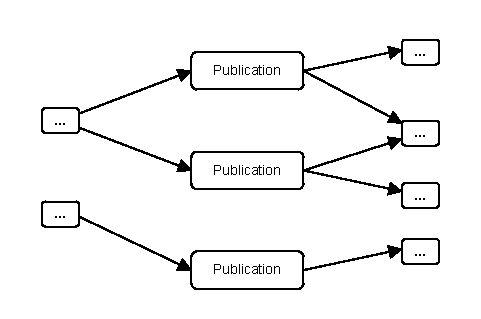
\includegraphics[width=0.75\textwidth]{figures/figures-RKG_structure.drawio.pdf}
    \caption[Example Structure of an RKG]{Example structure of an \gls{rkg}. Here, the information of interest is gathered as a subgraph around nodes of type \emph{Publication}. HubLink uses these subgraphs by encoding them as Hubs to perform targeted inference.}
    \label{fig:rkg_structure}
\end{figure}

When retrieving data from a graph, it is important to ensure that the relationships between information are retained correctly to avoid losing valuable data. This can be challenging, as it is not always clear how much of the surrounding information is actually needed \cite{peng_graph_2024,hu_grag_2024}. Our solution to this challenge is to decompose the graph into distinct \texttt{Hub} structures. This design choice is informed by the way information is organized within an \gls{rkg}. As observed by \textcite{verma_scholarly_2023}, an \gls{rkg} stores scientific data through research entities. Due to the inherent structure of graphs, related data tends to cluster around these entities. In this setup, the research entities act as roots, aggregating scientific information through their neighboring nodes. 

\autoref{fig:rkg_structure} illustrates this concept. It shows entities of the \emph{Publication} type that inherently store scientific information about the publication around them. In this case, each publication entity serves as a root, with its associated data stored in the surrounding nodes. Given that questions in scholarly \gls{kgqa} typically target information related to research entities, this natural clustering is exploited in the retrieval strategy of HubLink. We refer to this cohesive unit of information as a \texttt{Hub}, where each hub is based on a root node and encompasses all semantically related information accessible through paths originating from it.

Encoding these hubs in a vector space requires careful consideration of two key aspects: a) the significance of a node relative to the root node of the hub, and b) the preservation of relationships among the nodes within the hub. To meet both criteria, we consider all directed paths within the hub that start at the root and lead to end nodes. These paths are referred to as \texttt{HubPaths}. At the core, each \texttt{HubPath} represents a directed path within a hub that starts at the root entity of the hub, follows the direction of the graph, and either a) continues to the end of the graph, b) reaches a predetermined maximum length, or c) encounters a new root node of another hub. The idea of a \texttt{HubPath} is that the information on the path shares a common semantic meaning and should be encoded together in the vector space. Therefore, each \texttt{HubPath} is converted to vectors during indexing and stored in a vector database.


\subsection{Applying a Diversity Ranker on the Triple Level}

During development, we encountered an issue caused by retrieving triple-level vectors from the index. Since it is common that multiple triples $(s,p,o)$ share the same subject $s$, this leads to a situation where many irrelevant triples receive a high similarity score simply because they share the same subject. This creates a problem during retrieval in which only a fixed number of \texttt{HubPaths} are selected per candidate hub.
% The retrieved paths often add no value to answering the question because they all have the same subject entity, which by itself has a high relevance to the query, but the remaining information in the triple has not.

To illustrate this, consider the following question: \enquote{Which authors does the paper with the title 'A Complexity Metric for Microservices Architecture Migration' have?}. When this question is processed, it is decomposed into several components, one of which includes the paper title. Then, a similarity search is performed using these components. If the graph contains many triples where the title is the subject, these triples may dominate the top results due to the strong subject match, regardless of whether their predicates and objects are actually useful for answering the question. This effect can crowd out more relevant triples, such as those identifying the authors, from the top-k ranked \texttt{HubPaths} for a hub.

To mitigate this issue, we introduce a \emph{Diversity Ranker}. This component penalizes triples whose subject has already been encountered, thereby encouraging a more diverse set of \texttt{HubPaths} in the results. This increases the chances of retrieving paths that contribute novel and useful information. 

\subsection{Using Weighted Averaging for Scoring of Hubs}

In earlier stages of development, we calculated the score of a hub by taking the average of all associated \texttt{HubPath} objects. However, this approach revealed an issue that led us to adopt a weighted mean instead. Originally, the unweighted hub score was calculated as:

\[
\text{Score}(Hub) = \frac{1}{n} \sum_{i=1}^{n} \text{Score}(h_i), \quad h_i \in \mathcal{H}
\]

Here, \( \mathcal{H} \) denotes the set of all \texttt{HubPath} objects for a given hub, \( h_1, \dots, h_n \) are the individual paths, and \( n \) is the number of these paths. The main drawback of this method is that all paths are treated equally, regardless of their individual relevance. As a result, a hub with many average-quality paths could end up with a higher total score than a hub that has fewer but highly relevant paths. This leads to a situation where important paths with high scores are overshadowed by a large number of less relevant ones, even though they might be critical for the overall quality of the hub. To address this issue, we now use a weighted mean, where paths with higher scores contribute more significantly to the overall score of the hub. Formally, let \( \vec{s} = [s_1, s_2, \dots, s_n] \) be the list of scores of all paths for a given hub. The weights for this new calculation are computed as follows:

\[
w_i = \exp(\alpha \cdot s_i)
\]

The final weighted score of the hub is then given by:

\[
\text{Score}(Hub) = \frac{\sum_{i=1}^{n} w_i \cdot s_i}{\sum_{i=1}^{n} w_i}
\]

The parameter \( \alpha \) controls the extent to which high path scores are emphasized. Furthermore, this parameter can be fine-tuned to adapt to any given context. 


\subsection{Enriching Hubs by Linking to External Data}

Although representing information as a graph introduces structure and emphasizes semantic relationships, it also comes with a trade-off: a loss of textual detail. This occurs because textual content must be adapted to the \gls{rdf} format, which fragments information into triples, each capturing only a small portion of the original narrative. The goal of the linking process in HubLink is to complement the structured graph data with additional, richer context from external sources. This should enhance answer generation by providing more complete and informative responses.


To illustrate, consider a literature search scenario in which individual papers serve as the hub objects. Each hub is associated with a unique identifier, typically the DOI of the paper. This identifier enables the retrieval of additional information beyond what is captured in the graph. For example, we may connect to an external vector store that holds embeddings of the full-text from papers. Once relevant hub candidates are identified, the linking process uses their DOIs to perform targeted nearest-neighbor searches on these text embeddings. The returned text segments are then used to enrich the knowledge of the corresponding hubs. By combining structured graph data with context-rich textual extracts, this process can lead to more comprehensive and nuanced answers. In addition, it supports transparency in the retrieval process, as the enriched responses can be directly traced back to their source documents.



\subsection{Providing Two Different Retrieval Strategies} 

During the development of HubLink, we decided to implement two different retrieval strategies. This decision was driven by a trade-off that emerged during development. By introducing both strategies, we allow users to choose the strategy that best suits their specific use case. In the following, we take a closer look at this trade-off.

The first approach, \emph{direct retrieval}, enables fast retrieval using the vector index to quickly identify semantically similar content. Although this method is efficient and scalable, it becomes less effective in retrieving localized information as the size of the index grows. When multiple contexts from different sources share semantic similarity with the query, they may all be retrieved, regardless of whether they are relevant to the specific intent of the question. This can be problematic for questions that are meant to target particular segments of the knowledge graph.

To mitigate this limitation, traditional search systems often use metadata filters (e.g., research field, publisher, publication year) to narrow the scope of search results. HubLink incorporates a similar principle in its second strategy, \emph{graph traversal retrieval}. In this approach, a specific entry point in the graph, referred to as a topic entity, is used to constrain the search to a relevant subregion of the graph. Without such a focus, the system would need to search the entire graph, increasing the risk of retrieving irrelevant information from unrelated areas. Consequently, the topic entity effectively acts as a filter, making this strategy particularly valuable in large-scale graphs containing millions of nodes.

However, using the \emph{graph traversal retrieval} strategy comes with the drawback that a topic entity must be known or inferred. In some cases, such an entity may already be known. For example, if it is already known that a question refers to publications of a specific research field, the entity of that research field could be provided as input. Alternatively, the topic entity may be extracted automatically from the question, for example, through \emph{named entity recognition} as demonstrated in \cite{wang_reasoning_2024}. Here, the terms provided in the question are mapped to entities in the graph using an \gls{llm} process. 

Furthermore, another drawback of the \emph{graph traversal retrieval} strategy is that traversing the graph is time-consuming and adds computational expense. This is because the hubs must be found by traversing the graph, which is a complex process that can take a considerable amount of time depending on the size of the graph and the number of hubs. The time requirement increases even further if the initial hubs do not provide an answer, and deeper levels must be traversed. Thus, the trade-off between the two retrieval strategies becomes increasingly relevant as the graph grows in size: it is a balance between the accuracy of the results and the computational cost and runtime. Consequently, we decided not to enforce a one-size-fits-all solution. Instead, users should choose the strategy that best fits their specific use case and requirements.

\subsection{Prompt Engineering}

The HubLink algorithm includes a total of four prompts, which are presented in Appendix~\ref{sec:appendix:hublink_prompts}. During development, we observed that the performance of HubLink strongly depends on whether the prompts actually achieve the goal for which they are used. This is particularly true when generating partial answers. If the task description is too vague, too much irrelevant information will be included, and if it is too restrictive, too little information will be included. In the following, we briefly introduce our rationale behind each of the prompts in HubLink.

\paragraph{Partial Answer Generation Prompt} This prompt is responsible for creating a partial answer for each hub. It is important here that even if the hub does not fully answer the posed question, all partial information provided by the hub for the given answer is formulated into a partial answer. We therefore created a prompt that prioritizes the integration of partial information even if it is not yet apparent whether the information is actually useful for the final answer later on. To support the \gls{llm} in understanding the task, we created a few-shot prompt that demonstrates how partial answers should be created from the hub information.

\paragraph{Final Answer Generation Prompt} This prompt receives all created partial answers and generates a final answer by aggregating all partial answers. In addition, the \gls{llm} has the task of marking every fact in the answer with a source in the form of $[i]$. With this, we want to ensure that transparency about the information source is guaranteed during answer creation, which is particularly important in the scientific field. At the end of the generated answer, a list with the DOI and the title of the publication is appended.

\paragraph{Question Component Extraction Prompt} This prompt is used to extract the components of the question from the given query. Here, we created a few-shot prompt to show the \gls{llm} the desired granularity for extraction.

\paragraph{Triple Filtering Prompt} This is the last prompt in the execution. Here, based on the posed question, the answer, and the triples, a decision is made as to which triples are most relevant to the answer to filter out those triples that are not needed.

It should also be mentioned here that, depending on the application case, it may be reasonable to make adjustments to the current prompts. For example, during partial answer generation, the focus could be on identifying contradictions between sources instead of a simple synthesis of information.

\section{Generalizability and Scalability}
\label{sec:hublink_generality_and_chances}

The fundamental design of HubLink offers potential regarding its range of application and performance capabilities. This section discusses these aspects. First, we explain why we consider HubLink to be schema-agnostic. Then, we examine the adaptability of the approach to other domains. Last, we explore the scalability of the approach by discussing how the modularity of the approach facilitates efficient processing even on \glspl{kg} comprising millions of entities and relations.

\subsection{Why HubLink is Schema-Agnostic}
% This means that it does not make assumptions about the particular vocabulary or ontology used in the underlying \gls{kg} and consequently, does not rely on a fixed set of entity types or relation predicates. 
% Training based but schema agnostic: LLMs
% Training based and not schema agnostic: Semantic Parsing
% not schema agnostic: Semantic parsing with examples

We define \emph{schema-agnostic} as a characteristic of a system that does not rely on a fixed schema (i.e., a predefined set of classes, predicates, or relations). Instead, such a system operates on arbitrary or previously unseen graph structures without requiring adaptation of its core functionality.

HubLink is designed to be schema-agnostic because all core processing steps, including graph traversal, extraction, embedding, and retrieval, work on generic triples. Consequently, HubLink does not depend on any particular classes, property names, or specific ontology structures. This design makes the approach directly applicable to graphs with diverse or evolving schemas without necessitating changes to the underlying algorithms.

Nevertheless, the implementation of the \textsc{isHubRoot} classification function introduces a point where schema awareness can be incorporated, particularly if classification relies on entity types. The degree of sensitivity to schema evolution in such instances depends on the specific implementation chosen. For example, in the experimental setting conducted for this thesis, the \emph{Paper} type from the \gls{orkg} served as a criterion for \texttt{HubRoot} classification. We argue that this specific choice does not render the overall approach inherently schema-reliant. This argument is supported by two main points: first, the designated type is fundamental to the graph structure in that context and is not anticipated to undergo frequent changes. Second, the construction and retrieval of paths within hubs remain entirely independent of schema-defined types. Furthermore, as defined in Section~\ref{sec:hublink_hubroot_definition}, the HubLink approach supports alternative methods for classifying \texttt{HubRoots} that do not use any direct schema information from the graph, thus offering a mechanism to maintain schema independence even in the hub classification stage.


% Although schema information can optionally be used as a criterion for the \texttt{isHubRoot} classification function, this is not a requirement. Even if specific types are used to define which nodes serve as hub roots, the construction and retrieval of paths within those hubs remain entirely schema-agnostic. This ensures that HubLink can operate flexibly on heterogeneous graphs.

\subsection{Applicability to Other Domains}

Although the current implementation of HubLink has focused on \glspl{rkg}, which store scientific data, the approach is not limited to this domain. We believe that HubLink is broadly applicable to any field where the knowledge base is organized around well-defined entities. This includes domains such as internal company documents, Wikipedia articles, medical case records, or biological entities such as genes or proteins.

The key strength of HubLink lies in its ability to extract, aggregate, and retrieve information centered around specific objects. If these objects of interest are identifiable within the given data context, they can be used as hubs, making HubLink a flexible and adaptable solution across diverse domains. 

\subsection{Scalability to Large Graphs}

In addition to cross-domain applicability, scalability is a critical factor for the practical use of HubLink. Although large-scale evaluations fall outside the scope of this thesis, we argue that HubLink is well suited for deployment on \glspl{kg} containing millions of triples. This is because a unique advantage of HubLink lies in its modular, hub-based design. For queries that span multiple subgraphs or require aggregating information from distributed sources, the HubLink approach allows the graph to be decomposed into hubs. Each hub can then be individually evaluated to determine whether it contributes to answering the query. This allows the system to scale horizontally by distributing the evaluation across multiple hubs or even machines. This modular approach has the potential to handle complex queries efficiently by dividing the problem into smaller subproblems. We argue that HubLink opens up new possibilities for scalable and intelligent retrieval across large and complex \glspl{kg}. 

To realize the indexing of large-scale graphs, we propose two complementary strategies:

\paragraph{Indexing the entire Graph:} 
One possible strategy is to index the entire graph using the embedding-based method of HubLink. Since the vector similarity search does not scale linearly with the size of the graph, response times remain relatively stable even as the graph grows. However, this property applies exclusively to the \emph{direct retrieval} strategy because, in contrast, the \emph{graph traversal} strategy requires evaluating all hubs that can be reached from the topic entity. However, this makes the traversal strategy particularly effective for queries targeting a specific region of the graph, as the topic entity naturally constrains the retrieval scope, leading to more focused searches.

\paragraph{Partitioning the Graph:} 
An alternative approach that would also allow for control of the retrieval section involves partitioning the graph into multiple indices. This method proves advantageous when the relevant semantic domain of a query is known in advance. The underlying assumption is that large-scale \glspl{kg} can be divided into semantically coherent subgraphs. Once such segmentation is performed, indexing can be limited to the subgraphs that are relevant to the queries. Consequently, it becomes necessary to select the appropriate index before processing a question. This selection can be carried out manually or automatically, for example, through an \gls{llm}-based classification mechanism.

% To improve efficiency, the update process can be optimized by leveraging the timestamps of the modified triples, as only those paths affected by actual changes need to be removed and rebuilt, thereby avoiding the unnecessary reconstruction of unaffected components.

\section{Updating the Index}
\label{sec:updating_the_index}

The HubLink retriever can only respond to questions based on the information stored in the associated index. For this reason, it is essential to update the index whenever changes are made to the graph to ensure that the data remains consistent and up-to-date. The following section explains how this update process can be implemented.

As illustrated in the pseudocode of the function \textsc{hubIndexNeedsToBeUpdated}, changes in individual hubs can be detected by comparing the hash values of the current \texttt{HubPath} objects with those stored in the index. A mismatch indicates a modification and thereby signals the need for an update. Alternatively, if each triple in the graph is annotated with a timestamp indicating its last modification, this metadata can also serve as a criterion for determining whether an update is required. When a hub is identified as outdated, it can then be refreshed by invoking the \textsc{buildHubs} method. This procedure removes outdated entries from the index and rebuilds the corresponding \texttt{HubPaths}. 

The pseudocode in Section~\ref{sec:hublink_indexing} demonstrates how the index update can be implemented. This indexing function is designed to serve both initialization and maintenance purposes. During an update run, the algorithm iterates through each hub, verifying whether the paths stored in the graph remain consistent with those in the index. If discrepancies are detected, the affected components are updated accordingly. This procedure, which we refer to as the \emph{Fixed Update} strategy, entails a comprehensive review of the index performed at specified intervals. Although computationally intensive, this approach guarantees that the entire index is synchronized upon completion.

An alternative strategy is the \emph{Dynamic Update}, wherein updates are executed in real time in response to changes in the graph. When a modification occurs, the affected hubs are immediately updated using the \textsc{buildHubs} method. This method requires the integration of a monitoring routine that is automatically triggered upon any update to the graph. Such a routine can either invoke \textsc{buildHubs} directly or interact with the vector index to selectively adjust the relevant data entries.

In summary, we propose the following two strategies to maintain index consistency:

\begin{itemize} 
    \item \textbf{Fixed Update:} Involves a complete and periodic examination of the index to identify and refresh outdated hubs. This process is performed at predefined intervals and ensures full synchronization.
    \item \textbf{Dynamic Update:} Executes updates immediately following any modification to the graph. A monitoring routine initiates the update process, targeting only the affected components.
\end{itemize}



\section{Limitations}
\label{sec:hublink_limitations}

The primary limitation of HubLink is the requirement of an index. This index is crucial for inference because only the information stored in the index is seen by the retriever. Consequently, if a question asks for information that is not indexed as part of a hub, it is not considered. This requires careful management of the index, for which we outline several possibilities in Section~\ref{sec:updating_the_index}. Nevertheless, we argue that using an index instead of training is a considerable benefit, as building the index itself does not require any additional data but the graph itself.

Beyond the limitation of the index, several other considerations affect the HubLink approach. The definition of optimal criteria to classify \texttt{HubRoot} entities from which the hubs are built is not straightforward and depends on the underlying graph. If these criteria are not well defined, relevant information may not be encapsulated within hubs, rendering it unreachable until the criteria and index are updated.

Furthermore, the indexing process itself, particularly for large or frequently updated graphs, can be computationally intensive and time-consuming. In addition, the decomposition of paths into multiple vector representations during indexing contributes to increased storage requirements of the index. These factors introduce maintenance overhead, as changes in the graph necessitate updates to the HubLink index.

Moreover, the answer generation capabilities of HubLink are significantly dependent on the \gls{llm} utilized. Whether the \gls{llm} is able to pre-filter extraneous information during the generation of partial answers and subsequently synthesize these into a coherent final answer relies upon the performance of the \gls{llm} and also whether the prompts are clear and specific enough for the \gls{llm} to understand. This may require the adaptation of prompts for different \glspl{llm}, tasks, or domains to achieve optimal results.

Operational aspects also introduce limitations. For instance, the graph traversal retrieval strategy requires a topic entity as an input, which implies either user provision or an auxiliary mechanism for entity linking from the query. Additionally, HubLink is an embedding-based system at its core and, as such, inherits certain limitations common to these types of systems. For example, as described by \textcite{wang_reasoning_2024}, the processing and interpretation of numerical constraints, such as dates, value ranges, or specific metric comparisons, presents challenges for such systems.

% If the information that is asked for is not indexed as part of a hub, it can't be found by the retriever. This is a limitation of the retrieval process, as the retriever can only find information that is part of a hub.

% The definition of the optimal criteria to classify HubRoots is not straightforward, as it depends on the underlying graph ontology. If the criteria is not well defined, relevant information might not be encapsulated within hubs, making it undiscoverable during retrieval.

% If new types of entities or relationships are added into the RKG, and they do not fit the existing HubRoot classification criteria or are not part of any current hub, they will not be indexed and thus the system will not be able to retrieve information about it until the HubRoot criteria is updated.

% Especially for large graphs, the indexing process can be computationally expansive and time-consuming. Future graph updates necessitate an update to the index. If these updates are frequent this can lead to a significant overhead. Furthermore, as a graph provider, in addition to the graph itself, the index of HubLink has to be managed as well which adds further maintenance costs.

% The decomposition of paths during the indexing process increases the size of the index requiring more overall storage.

% The answer generation heavily depends on prompt engineering. It is important that during the generation of partial answers, the LLM pre filters unnecessary information and moves forward those information that could potentially be relevant for the final answer. Consequently, the generation of the final answer needs to be able to synthesize all relevnt information from the partial answers, which depends on the prompt engineering instructions. COnsequently, it might be necessary to adapt the prompts for specific tasks as a general prompt might not be sufficient for all scenarios.

% The graph traversal strategy requires a topic entity as input. This requires either the user to provide such an entity or a automatic procedure that maps the question to an appropriate entity in the graph. An example for such an approach can be found in the work of \textcite{wang_reasoning_2024}.

% For complex queries or in dense graph regions, the number of candidate hubs and paths can become very large, impacting the performance of ranking, pruning, and subsequent LLM processing steps.

% The processing of numerical constraints, such as dates, ranges of values or specific metric comparisons, presents a potential challenge for embedding-based retrieval approaches like HubLink, as highlighted in previous research \cite{jin_floating-point_2024}.


